Model \smod je napsán v programovacím jazyce Python. Příprava dat a samotný výpočet v časové smyčce jsou od sebe odděleny. Příprava dat využívá v současné době nástroje z knihoven ArcGIS, což byl jeden z primárních důvodů volby  programovacího jazyka Python, který je pro prostředí ArcGIS nativním skriptovacím jazykem. Proces samotného výpočtu již využívá pouze standardní knihovny Python, jako je knihovna \texttt{numpy}, nebo \texttt{math}, atd. Následující text je rozdělen do čtyř částí, které popisují instalaci modelu (kapitola~\ref{kap:instalace}), vstupní data (kapitola~\ref{kap:vstupy}), tok programu (kapitola~\ref{kap:tok}) a výstupy z modelu (kapitola~\ref{kap:vystupy}). \\
% 
% 
\rule{\textwidth}{0.3pt}

%%%%%%\subsubsection{Princip výpočtu} \label{kap:principvypoctu}
%%%%%%\input{./text_cz/mat_a_met/CZsmoderp_princip}
%         


	\section{Instalace \smod a spištění v ArcGIS} \label{kap:instalace}
	  
  Uživatel má několik možností, jak používat model \smod. Pomocí instalačního souboru lze nainstalovat \smod jako běžný Python balíček. Model \smod je rovněž poskytován ve formě zdrojového kódu. Je tedy možné spouštět balíček přímo bez instalace. V této části manuálu je popsán první a nejjednodušší způsob, instalace pomocí instalačního souboru. 
  
  Model \smod je distribuován pod GPLv3\footnote{Více informací na: \href{https://www.gnu.org/licenses/gpl-3.0.en.html}{gnu.org/licenses/gpl-3.0.en.html}} licencí. Veškeré stažitelné materiály lze stáhnout na webových stránkách Katedry hydromeliorací a krajinného inženýrství, Fakulty stavební ČVUT v Praze~(\href{http://storm.fsv.cvut.cz/cinnost-katedry/volne-stazitelne-vysledky/smoderp/}{storm.fsv.cvut/../smodep/}). Na odkazu lze stáhnout malíček modelu \smod, instalační EXE soubor, tento manuál a další aktuální informace. 
  
  Instalační soubor pro operační systém Windows lze stáhnout na adrese~\href{http://storm.fsv.cvut.cz/cinnost-katedry/volne-stazitelne-vysledky/smoderp/program-smoderp2d/}{storm.fsv.cvut/../smodep/program-smoderp2d/} na odkazu: Instalační EXE soubor pro Windows. Po spuštění souboru se otevře průvodce k instalaci standardního balíčku Python (úvodní obrazovka průvodce je ukázána na obrázku~\ref{fig:pruvodce}). Po ukončení instalace lze model \smod importovat do Python skriptu příkazem {\tt import smoderp2d.main}. 

  Před použitím modelu se doporučuje provést test, který ověří, zda má uživatel nainstalované ostatní používané balíčky. Testovací skript je spolu s testovacími daty ke stažení na adrese ~\href{http://storm.fsv.cvut.cz/cinnost-katedry/volne-stazitelne-vysledky/smoderp/program-smoderp2d/}{storm.fsv.cvut/../smodep/program-smoderp2d/} na odkazu: Test po instalaci. Testovací skript s názvem {\tt importrun.py} uložte do společné složky s testovacími daty {\tt test-data}. Po spuštění skriptu se otevře okno terminálu příkazové řádky. Pokud instalace balíčku \smod neproběhla nebo proběhla chybně, vypíše testovací skript hlášení ukázané na obrázku~\ref{fig:importerror}. Pokud nejsou nainstalované jiné nezbytné balíčky, může se chybové hlášení lišit. Pokud například chybí balíček {\tt numpy}, vypíše se na třetí řádek hlášení: {\tt No module named numpy}. V takovém případě je nutné chybějící balíčky doinstalovat běžným způsobem. Pokud proběhne testovací běh modelu \smod bezchybně, proběhne v okně terminálu hlášení ukázané na obrázku~\ref{fig:testok}. Výstupní soubory jsou pak uložený do složky {\tt test-out} v adresáři kde je uložen skript {\tt importrun.py}. V tento moment je model \smod včetně nezbytných balíčků zdárně nainstalován a je připraven k použití.
  
  \begin{figure}[t!]
    \centering
    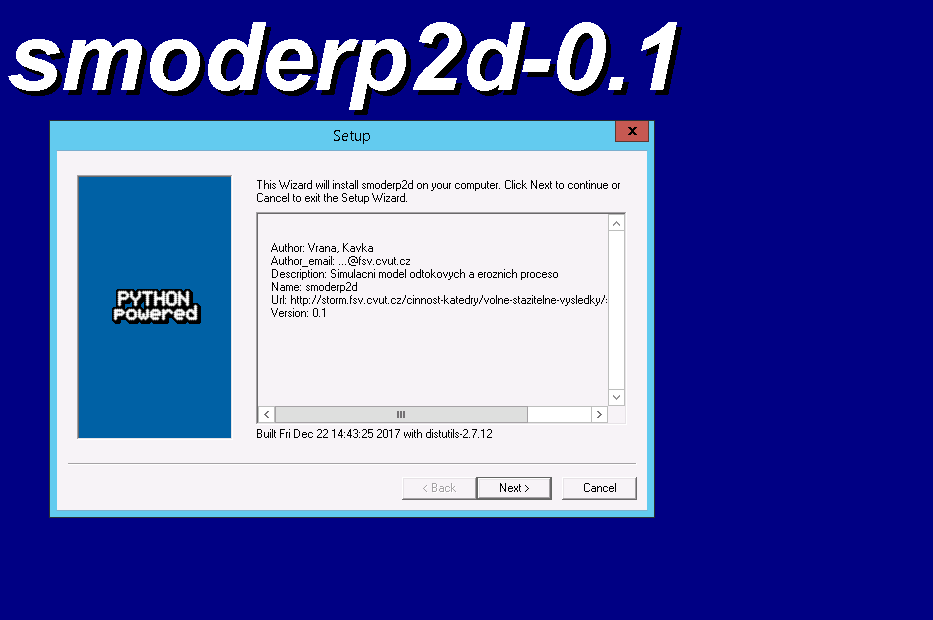
\includegraphics[width=0.75\textwidth]{./img/instalace.png}
    \caption{Úvodní obrazovka při instalaci balíčku \smod}
    \label{fig:pruvodce}
  \end{figure}
% 
  \begin{figure}[b!]
    \centering
    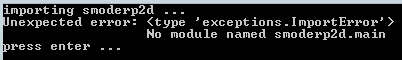
\includegraphics[width=0.75\textwidth]{./img/importerror.png}
    \caption{Hlášení při chybné instalaci balíčku modelu \smod}
    \label{fig:importerror}
  \end{figure}
% 
  \begin{figure}[t!]
    \centering
    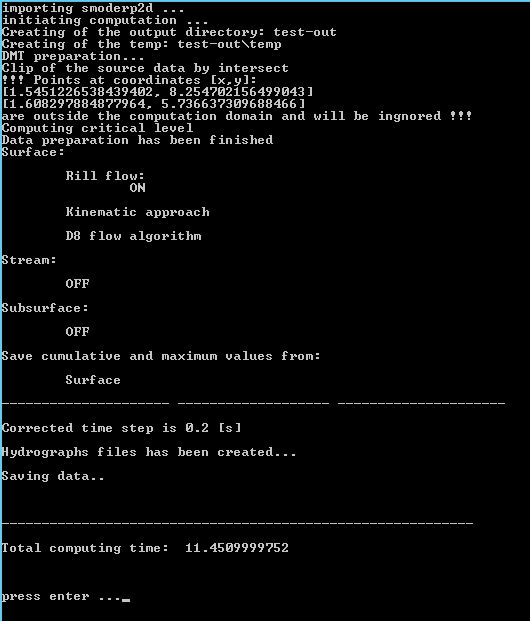
\includegraphics[width=0.75\textwidth]{./img/testok.png}
    \caption{Zdárný průběh testovacího skriptu modelu}
    \label{fig:testok}
  \end{figure}
  
\subsection{Použití modelu v ArcGIS}
  
  Současná verze modelu \smod využívá k přípravě vstupních dat výhradně software ArcGIS a Python balíček {\tt arcpy}. Proto je potřeba vytvořit spouštěcí skript, který načte a spustí model \smod. Takový skript může obsahovat následující příkazy:
%   \begin{figure}[h!]
    \begin{lstlisting}
      import smoderp2d.main as sm
      sm.run()
    \end{lstlisting}
%     \caption{Skript pro spuštění modelu \smod}
%   \end{figure}
  {\tt import smoderp2d.main as sm}  načte balíček modelu \smod. Spuštěním metody  {\tt sm.run()} je spuštěn samotný model. 
  
  Pro použití modelu v prostředí ArcGIS je třeba vytvořit ArcGIS {\tt toolbox}, kde je nastavený jako zdrojový soubor  uložený spouštěcí skript. Další krok je nastavení parametrů ArcGIS {\tt toolbox} odkud se načítají vstupní parametry do modelu. Pořadí zadávaných hodnot je {\bf nutné dodržet}! Ukázka ArcGIS {\tt toolbox} a vysvětlení parametrů je ukázáno na obrázku~\ref{fig:toolbox}. Připravený ArcGIS {\tt toolbox} a spouštěcí skript lze stáhnout na adrese~\href{http://storm.fsv.cvut.cz/cinnost-katedry/volne-stazitelne-vysledky/smoderp/program-smoderp2d/}{storm.fsv.cvut/../smodep/program-smoderp2d/} na odkazu: Použití modelu v ArcGIS. Detailnější popis vstupních hodnot je v kapitole~\ref{kap:vstupy}.
  
  
  
  \begin{figure}[t!]
    \centering
    \begin{minipage}[t]{.45\textwidth}
      \centering
      \vspace{0pt}
      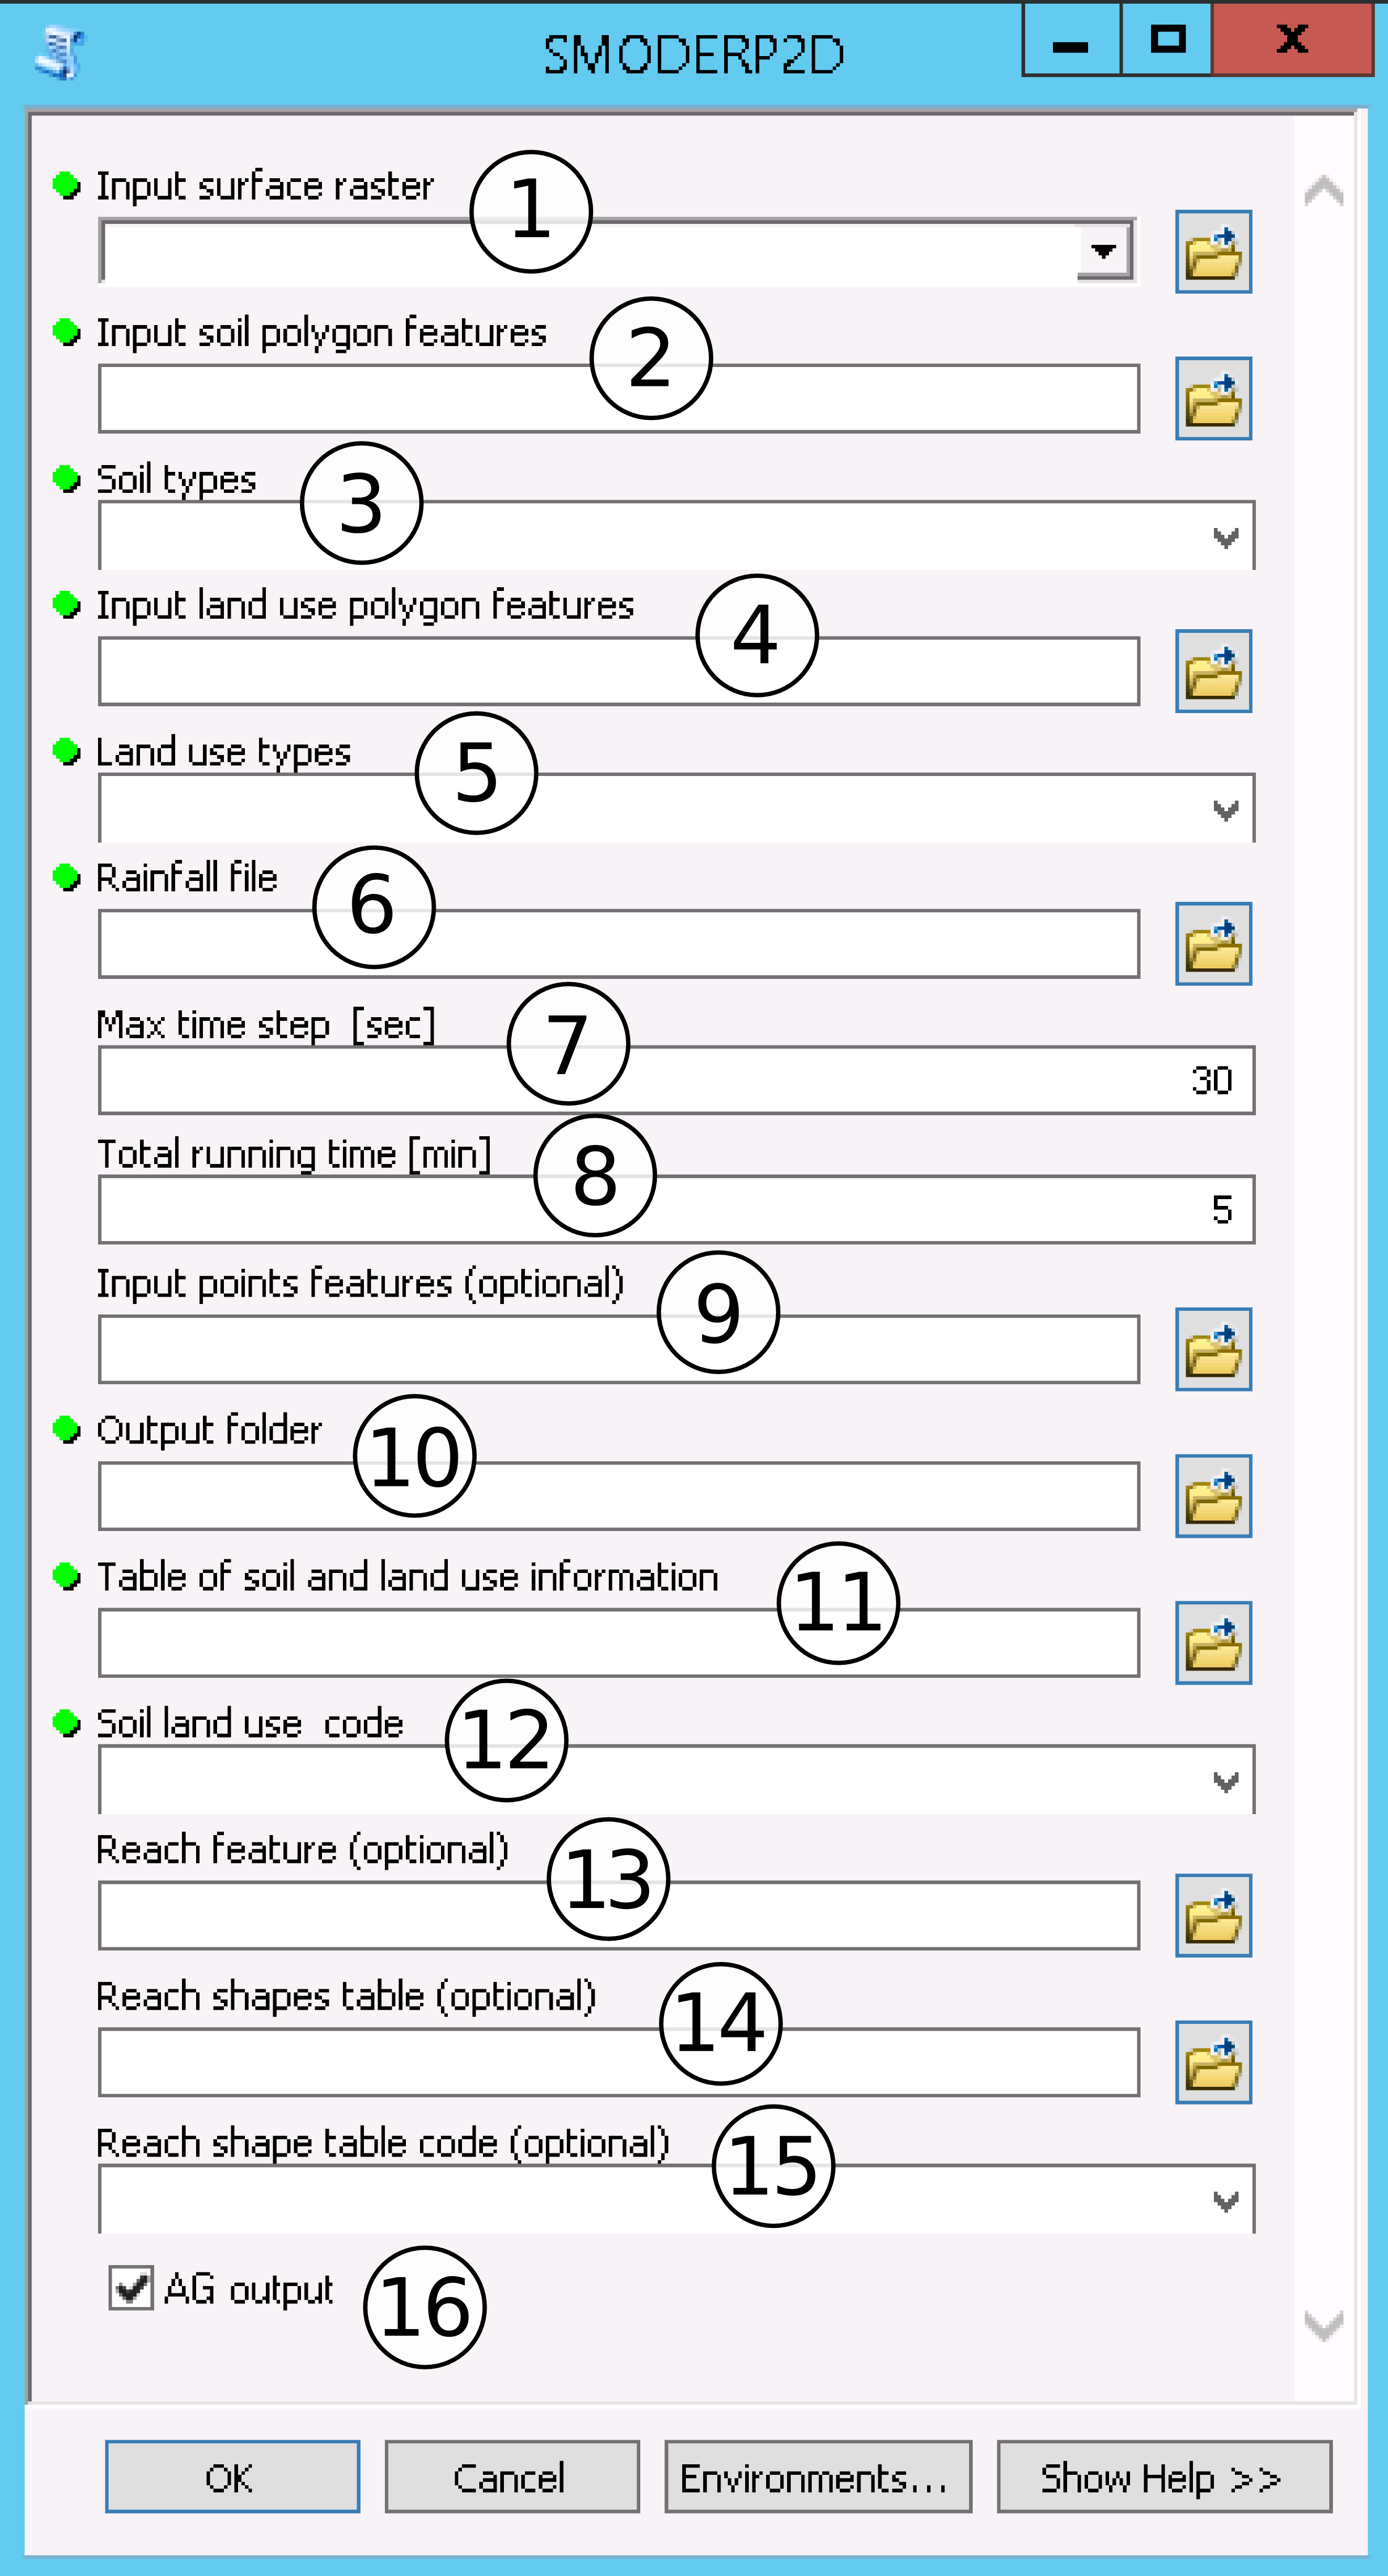
\includegraphics[width=\textwidth]{./img/toolboxpopis4.png}
    \end{minipage}\hfill
    \begin{minipage}[t]{.55\textwidth}
      \centering
      \vspace{0pt}
      {\scriptsize\sffamily
      \begin{tabular}{lp{.5\textwidth}l}
                     & Popis                                       & ArcGIS typ dat     \\
        \hline
	\circled{1}  & Cesta k digitálnímu modlu terénu            &  {\tt Raster layer} \\
	\circled{2}  & Cesta k vektorové vrstvě rozložení typu půd &  {\tt Shapefile} \\
	\circled{3}  & Název pole s id typů půd &  {\tt Field} \\
	\circled{4}  & Cesta k vektorové vrstvě využití území &  {\tt Shapefile} \\
	\circled{5}  & Název pole s id využití území &  {\tt Field} \\
	\circled{6}  & Cesta k souboru se srážkovými daty &  {\tt Text file} \\
	\circled{7}  & Maximální časový krok &  {\tt Double} \\
	\circled{8}  & Konečný čas výpočtu &  {\tt Double} \\
	\circled{9}  & Vrstva bodů pro výpis hydrogramů &  {\tt Shapefile} \\
	\circled{10} & Výstupní adresář &  {\tt Folder} \\
	\circled{11} & Tabulka s parametry modelu &  {\tt Table} \\
	\circled{12} & Označení pole v tabulce \circled{11} &  {\tt Field} \\
	\circled{13} & Cesta k vrstvě linií hydrografické sítě &  {\tt Feature Class} \\
	\circled{14} & Cesta k tabulce s geometrií úseků hydrografické sítě &  {\tt Table} \\
	\circled{15} & Název společného pole pro spojení \circled{13} a \circled{14} &  {\tt Field} \\
	\circled{16} & Volba formy výstupních souborů &  {\tt Boolean} \\
      \end{tabular}
      }
    \end{minipage}
    \caption{ArcGIS {\tt toolbox} a vysvětlenými parametry}
    \label{fig:toolbox}
  \end{figure}
%     \centering
%     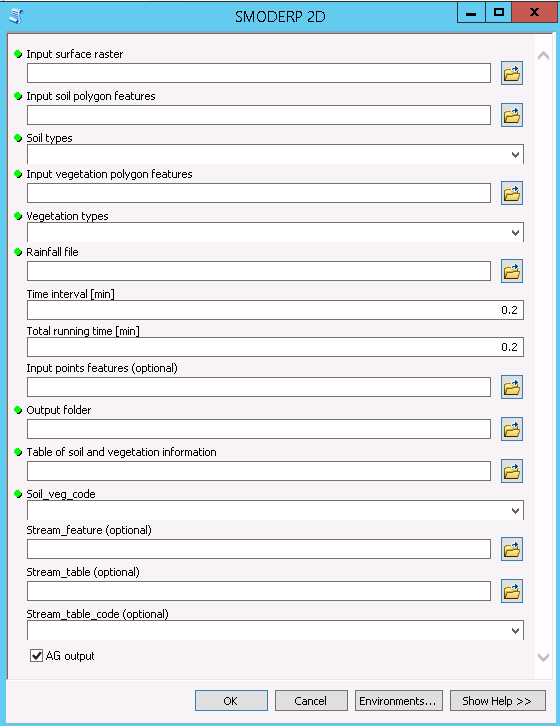
\includegraphics[width=0.75\textwidth]{./img/toolbox.png}
  
  
  
  
   
	
	
	\section{Vstupy do modelu} \label{kap:vstupy}
	%%!TEX ROOT = ../mainCZ.tex



Do modelu vstupují informace o topografii řešeného území, informace o typech půd a využití území a o jejich prostorovém rozmístění, informace o srážce, případně o geometrii dočasné hydrografické sítě.
Tato data jsou zadávána ve třech formátech: rastrovém, vektorovém a textovém. 
% Do modelu vstupují informace o topografii řešeného území, informace o typech půd a vegetaci, informace o srážce atd. 
Základní formát vektorových dat je formát shapefile. Tento vektorový formát byl vytvořen firmou ESRI, ale je zpracovatelný i jinými GIS softwary. Parametry modelu jsou uloženy v atributové tabulce pod specifickým názvem pole. 
% Shapefile popisuje prvky jako body, linie nebo polygony. Každý prvek má obvykle nějaký atribut, který ho popisuje jako v tomto případě jméno, či typ půdy. 
V následujícím textu jsou popsány náležitosti vstupních dat. 
% 
% Model pracuje s následujícími vstupy
Přehled vstupů do modelu je ukázán v tabulce~\ref{tab:vstupy}.


% 

% 
\begin{sidewaystable}
% \begin{table}[]
\centering
\caption{Tabulka s přehledem vstulních dat modelu}
\label{tab:vstupy}
\small{
% \begin{tabular}{p{4cm}lp{2cm}p{5cm}}
\begin{tabular}{p{0.30\textwidth}lp{0.10\textwidth}p{0.30\textwidth}l}
\hline \hline
Název                              & Typ dat                       & Povinný / volitelný & Poznámka                                                                                      & Více v kapitole                                                 \\ \hline 
digitální model terénu             & raster                        & Povinný           & Touto vrstvou se řídí i prostorová diskretizace.                                                 & \ref{sec:vstupdmt}                                           \\ 
prostorové rozložení půd           & vektor - polygony             & Povinný           & V atributové tabulce identifikátor typu půdy.                                               & \ref{sec:vstuppuda}                                          \\ 
prostorové rozložení využití území & vektor- polygony              & Povinný           & V atributové tabulce identifikátor využití území.                                           & \ref{sec:vstupvegetace} a \ref{sec:upravatabulkyparametru}   \\ 
srážková data                      & .txt soubor                   & Povinný           & Kumulativně zadaná srážka.                                                                       & \ref{sec:vstupsrazka}                                        \\ 
maximální časový krok              & reálné číslo                  & Povinný           & Model mění délku časového podle odtokových podmínek; doporučuje se 30 - 60 sekund.               & \ref{sec:vstupkrok}                                          \\ 
výstupní adrešář                   & text                          & Povinný           & Adresář k uložení výsledků (při spuštění výpočtu se obsah adresáře vymaže!).                            & \ref{sec:vstupadresar}                                       \\ 
bodové výstupy hydrogramů          & vektor - body                 & Volitelný         & Body pro výpis výsledků.                                                                   & \ref{sec:vstupbody}                                          \\ 
% typ výpočtu                        & text                          & Povinný           & Uživatel má na výběr: pouze plošní odtok, plošný i rýhový odtok, plošný, rýhový odtok i odtok hydrografickou sítí               & \ref{sec:vstupryhovy}          \\ 
% volba výcesměrného odtoku          & logická proměnná              & Povinný           & Jednosměrný (výchozí)  nebo vícesměnný odtok                                                           & \ref{sec:vstupvicesmerny}      \\ 
paramtry půdy a využití území           & tabulka                       & Povinný           & Tabulka parametrů půdy a využití území. Názvy sloupců mají definované označení. Hodnoty se spojí s vektorovými vrstvami.            & \ref{sec:upravatabulkyparametru}\\ 
hydrografická síť                  & vektor - linie                & Volitelný         & Prostorové rozložení hydrografické sítě. Atributová tabulka obsahuje identifikátor tvaru jednotlivých úseků.        & \ref{sec:vodnitoky}             \\ 
parametry úseků hydrografické sítě       & tabulka                       & Volitelný         & Tabulka parametrů jednotlivých úseků hydrografické sítě.                                                                        &  \ref{sec:vodnitoky}     \\ 
volba arcgis výstupů               & logická proměnná              & Povinný           & Výchozí formát výstupních rastrů je proprietární formát ERSI. Uživatel může zvolit textový formát ASCII.                       & --- \\ \hline \hline
\end{tabular}
}
% \end{table}
\end{sidewaystable}
% \begin{itemize} \itemsep 0pt
% \item digitální model terénu
% \item shapefile půd
% \item shapefile využití území
% \item srážkový soubor
% \item časový krok výpočtu a celková doba simulace
% \item výstupní adresář
% \item bodová vrstva pro generování hydrogramů
% \item výstupní adresář
% \item typ výpočtu
% \item volba výcesměrného odtoku
% \item tabulka půd a vegetace a kód pro připojení
% \item shapefile hydrografické sítě
% \item tabulka vodních toků a kód pro připojení
% \item volitelné formy výstupů
% \end{itemize}

% 
% \pozn{
% \textbf{Nutno dodělat}
% \begin{itemize} \itemsep 0pt
% \item upravit podle aktuálního stavu
% \item upravit a zjednosušit tuto kapitolu
% \item propojit s tabulkama co jsou jinde v textu
% \item vložit sem tabulky parametrů výpočtu pokud nejsou jinde
% \end{itemize}
% }
% 
% 
% 
% 
% 
% 









\subsection{Digitální model terénu} \label{sec:vstupdmt} 

Rastr digitálního modelu terénu DMT, či anglicky DTM (Digital Terrain Model) reprezentuje souvislou morfologii určité části Země. DMT rastr je složen z jednotlivých buněk obsahující informaci o elevaci terénu.  Velikost buněk se liší v závislosti na velikosti zobrazovaného území. Pro účely modelu \smod by minimální velikost buněk měla být 2 metry, optimum je však 5 metrů a více. Model byl testován na rastrech o velikosti od několika málo do stovek tisíc buněk. DMT jednoho z testovacích povodí, povodí Nučice, obsahuje přes 125 tisíc buněk při velikosti buňky 5 $m$. Příklad DMT dalšího testovacího povodí Býkovice je ukázán na obrázku~\ref{fig:dmt}.


% 
% \begin{figure}
%   \centering
%   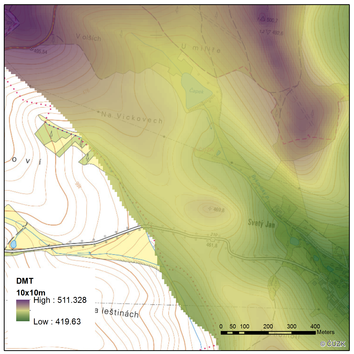
\includegraphics[width=0.5\textwidth]{./img/DMT_byk.png}
%   \caption{Výřez digitálního modelu terénu povodí Býkovice}
%   \label{fig:bykovicedmt}
% \end{figure}

 
 
 
 
 
 
 
 
 
 
 
 
 
 
 
 
 
 
 
\subsection{Půdní data} \label{sec:vstuppuda}


Vstupem do modelu je vektorová vrstva s vymezením jednotlivých půd.

Z hlediska půdních dat jsou obecně v ČR v rozumném měřítku podrobnosti k dispozici několik datových zdrojů. prvním je syntetická půdní mapa v měřítku 1:250 000 (KPP250), která vychází z komplexního průzkumu půd, tento datový podklad byl odvozen z předešlé tištěné mapy, čemuž také odpovídá měřítko podrobnosti dat. Po rozdělení půdního fondu na lesní a zemědělskou půdu jsou dalšími zdroji oddělené databáze pro tyto dvě skupiny. Na zemědělské půdě je dostupná půdní typologie (ve formě kódu BPEJ, resp. HPJ),  v současné době uvolněná k využití na portálu SPÚ. Prakticky neexistuje vhodný převodní klíč mezi hodnotami BPEJ a parametry infiltračních rovnic. Půdní druhy vyjadřující zrnitost ornice a podorničí podle Novákovy klasifikace je možné získat na VÚMOP v.v.i., dle aktuálního ceníku jako vektorovou vrstvu ve formátu shp. Dále jsou na portálu kpp.vumop.cz dostupné informace o konkrétních půdních sondách průzkumu KPP (kpp.vumop.cz).

V případě lesních půd, lesnické typologie a informací o půdních charakteristikách je dostupnost dat omezená. Veřejně dostupné jsou kódy lesnické typologie, ale metodika pro převod kódované informace na hydrologické vlastnosti půd (Macků, 2012) není dohledatelná. Hloubka lesních půd, zrnitostní složení a některé další charakteristiky jsou k dispozici na Ústavu pro hospodářskou úpravu lesů (ÚHUL), ale jejich poskytnutí vyžaduje součinnost s uvedeným úřadem. 

V případě využití modelu jsou klíčovým vstupem hydraulické charakteristiky půd, zejména nasycená hydraulická vodivost \acs{Ks}. Tato veličina je závislá na řadě půdních charakteristik, nejčastěji je vztahována k jejímu zrnitostnímu složení. Regionalizované informace o zrnitosti půd lze v ČR získat z výše jmenovaných datových zdrojů. 

Kromě dostupnosti prostorových dat vstupuje další komplikace v podobě nesouladu v klasifikaci půd na lesní půdě (USDA) a zemědělské (Novákova klasifikace). Syntéza těchto dat není triviální.
Průměrné hodnoty \acs{Ks} pro jednotlivé zrnitostní třídy, tzv. pedotransferové funkce, jsou odvozené z rozsáhlých půdních databází, které lze nalézt zejména v zahraniční literatuře \citep{wosten1999, toth2015}. V českých podmínkách je k dispozici, počtem analyzovaných vzorků značně omezená, databáze HYPRES-CZ \citep{mihalikova2013}. Obecně se však jedná o velmi variabilní data. Vzhledem k enormnímu rozptylu hodnot je pro snížení nejistot v hydrologickém modelování velmi žádoucí zajistit alespoň základní půdní rozbor v řešené lokalitě.


Obrázek~\ref{fig:puda} ukazuje výřez připravené vrstvy. Pro určení charakteristik je nutné, aby atributová tabulka dané vrstvy obsahoval identifikátor půdního typu. Identifikátor odkazuje na půdní charakteristiky, které jsou ale uložené v samostatné tabulce (viz níže). Mezi půdní charakteristiky a parametry používané modelem patří: \acs{HyVod} - \acl{HyVod}; \acs{Sorb} - \acl{Sorb}; \acs{n} - \acl{n}, \acs{b} - \acl{b}, \acs{X} - \acl{X} a  \acs{Y} - \acl{Y}. Hodnoty těchto parametrů lze převzít z tabulky~\ref{tab:kriticke} v příloze~\ref{sec:priloha}. Fyzikální význam těchto parametrů a jejich implementace v modelu jsou popsány v části~\ref{cast:1} toho manuálu. 





 
 
 
 
 
 
 
 
 
 
\subsection{Data využití území} \label{sec:vstupvegetace}
Obdobně jako u půdních dat je vstupem vektorový shapefile popisující využití území.

Data o využití území jsou dostupné jak ve vektorové, tak rastrové podobě. Na stránkách MŽP je po registraci zdarma dostupná vrstva CORINE LandCover. Ve větším detailu je možné data o povrchu odvodit z databáze ZABAGED. Z vrstev je možné získat informace o plochách, liniových prvcích, cestní síti, vodních tocích. Využití území je možné na zemědělské půdě zpřesnit na základě dat LPIS. Převod liniových prvků na plošné je vhodné jen u prvků šířky srovnatelné se zvoleným rozlišením DMT, např. u dálnic a silnic první třídy. Rozumnou volbou podrobnosti účely hydrologického modelování je spojení vstupních vrstev do přiměřeného množství kategorií. Vhodné členění může být například:  
\begin{itemize} \itemsep -3pt
  \item orná půda,
  \item travní porosty,
  \item ostatní zeleň,
  \item vodní plochy,
  \item sady,
  \item křovinaté porosty,
  \item lesní porosty,
  \item antropogenní a zpevněné plochy,
  \item zahrady.
\end{itemize}
V kategorii zpevněných ploch jsou zařazeny jak oblasti zástavby, tak zpevněné komunikace s přiměřeným rozšířením podle kategorie silnice. 
\pozn{????Orientační hodnoty poměrné plochy listové (Ppl), potenciální intercepce (Pi), povrchové drsnosti a retence jsou uvedeny v příloze.
}

Shapefile popisující využití území je ukázán na obrázku~\ref{fig:LU}. Obdobně jako u půd v předchozí sekci je třeba atributovou tabulku tohoto shapefilu doplnit o identifikátor daného využití území. Tento identifikátor odkazuje na charakteristiky daného povrchu definované ve zvláštní tabulce (popsáno v sekci~\ref{sec:upravatabulkyparametru}). Parametry související s využitím území, které vstupují do modelu jsou \acs{PotI} - \acl{PotI} a \acs{Lai} - \acl{Lai}. Jejich konkrétní použití je popsáno v části~\ref{cast:1} toho manuálu. 
% 
% \begin{figure}
%   \centering
%   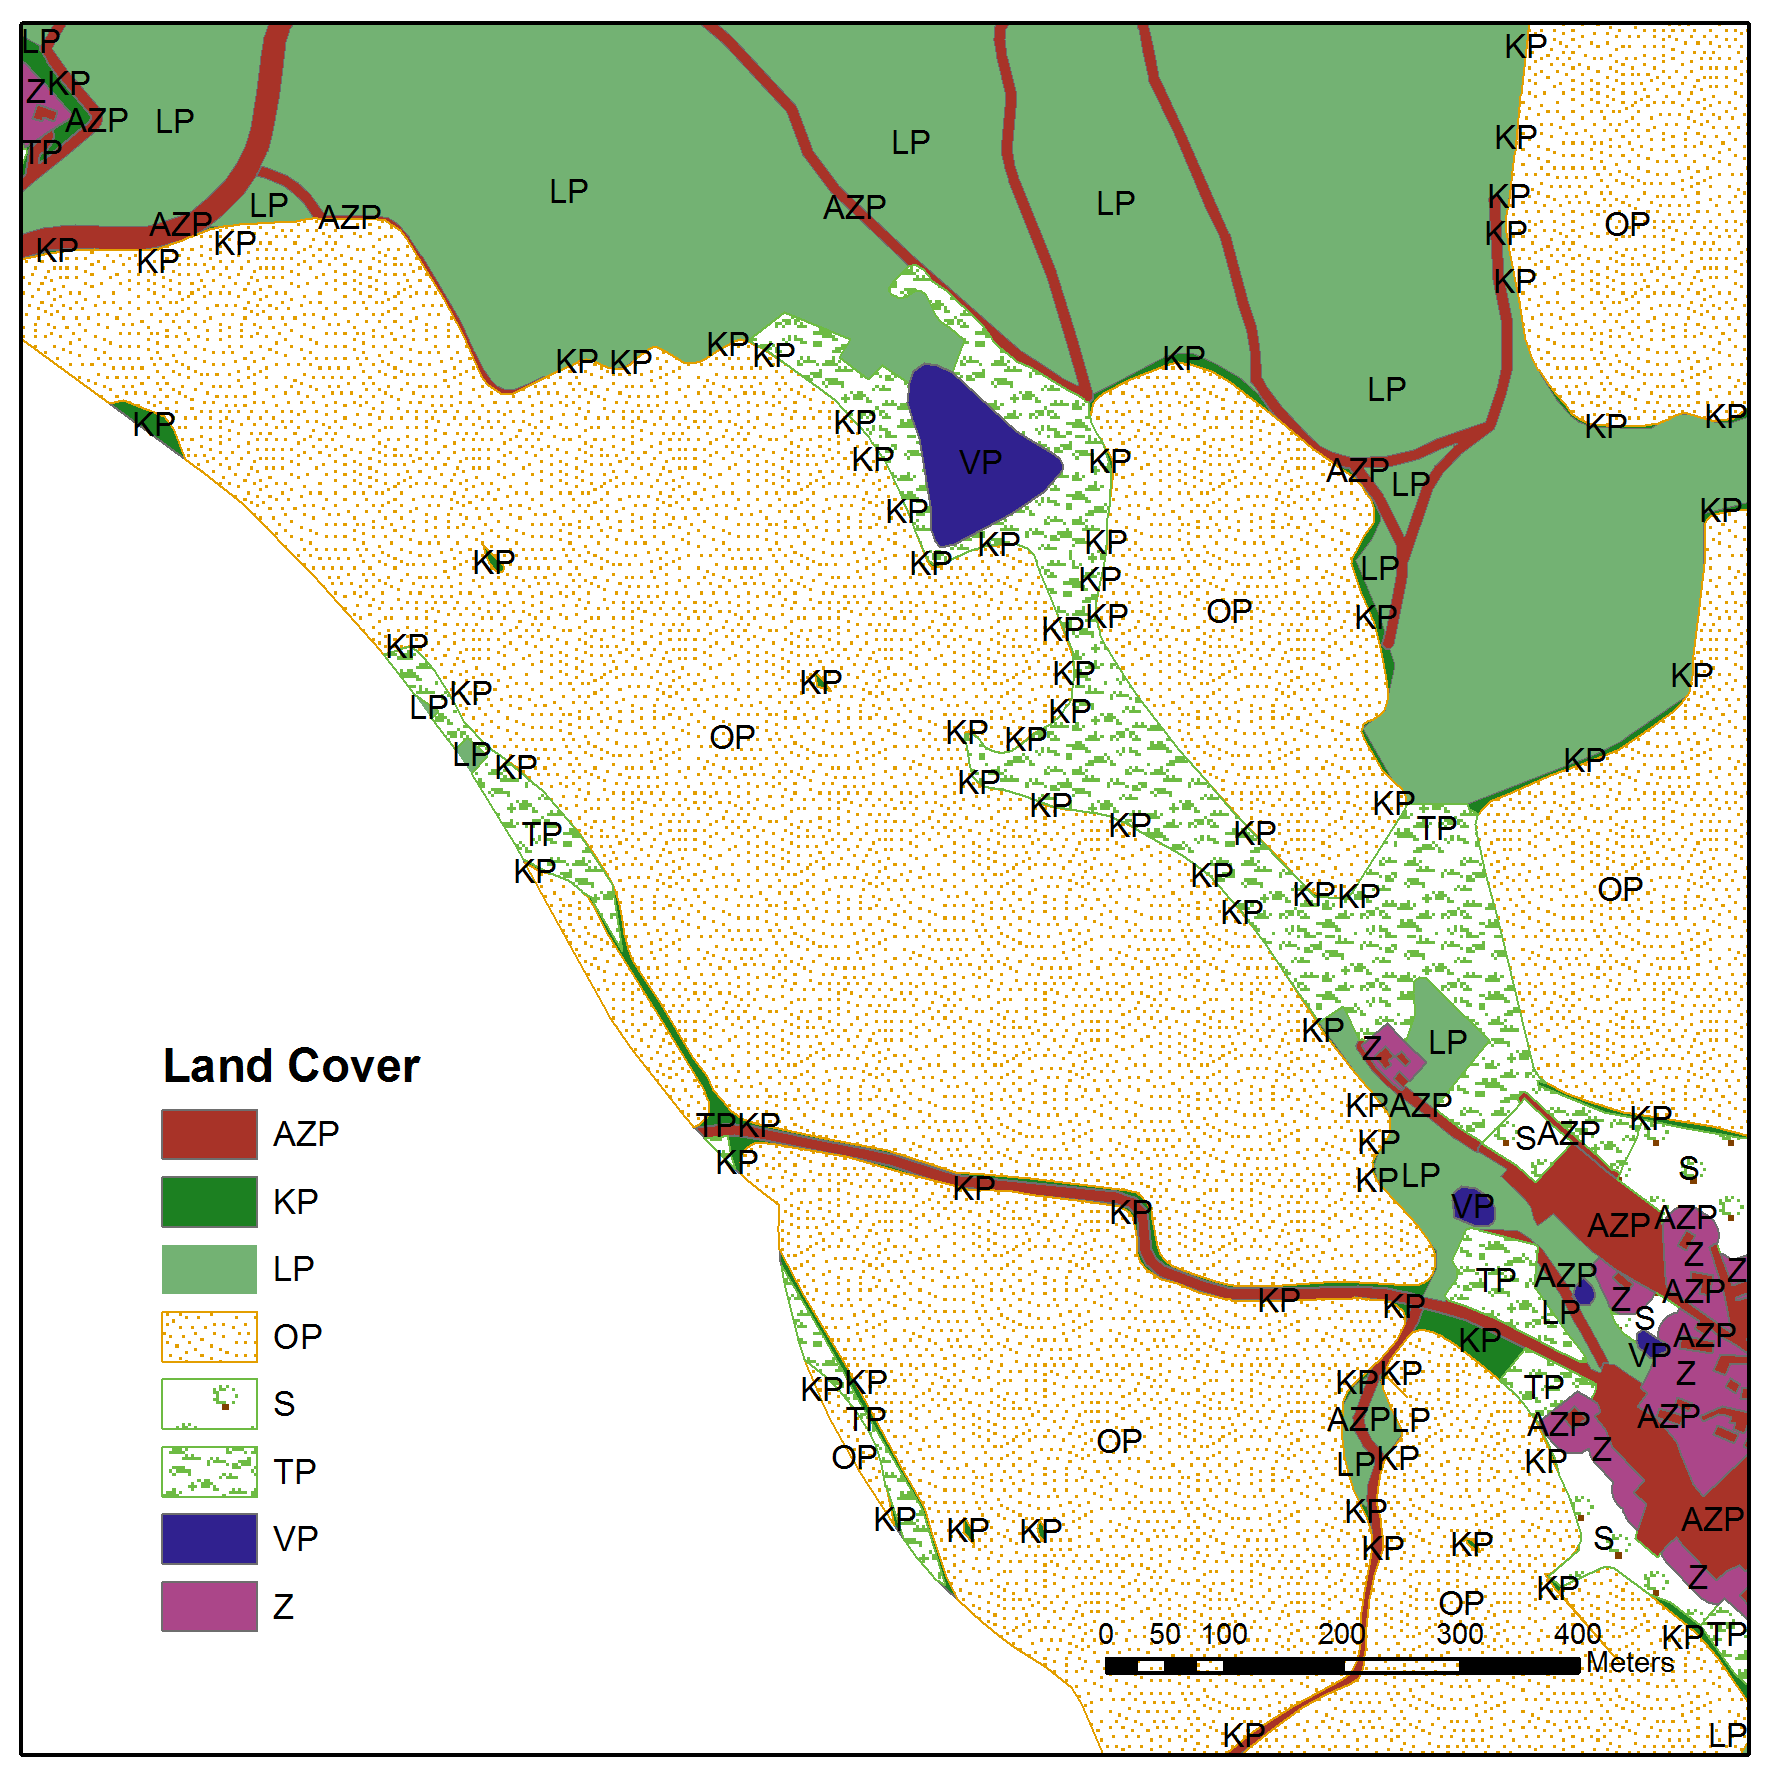
\includegraphics[width=0.5\textwidth]{./img/LandCover.png}
%   \caption{Ukázka vektorové vrstvy využití území -  Land Cover}
%   \label{fig:bykovicevegetace}
% \end{figure}
% 
% 
% 















\subsection{Tabulka parametrů půdy a využití území}  \label{sec:upravatabulkyparametru}

Další povinný vstup je tabulka, která obsahuje hodnoty jednotlivých parametrů popsaných v předešlých kapitolách a v části~\ref{cast:1} toho manuálu. Na tuto tabulku se odkazují identifikátory půdního typu a typu využití území definované pro jednotlivé polygony v atributových tabulkách vektorových vstupů. Tato tabulka může být do modelu vložena jako textový soubor. Na obrázku~\ref{fig:soilvegtablo} je ukázán příklad takové tabulky. V prvních dvou sloupcích jsou identifikátory ($id$) typu půd ($Soil$) a typu využití území ($Land$ $Co.$). Spojením těchto dvou $id$ jsou označeny parametry pro danou kombinaci typu půdy a využití území (třetí sloupec v tabulce na obrázku~\ref{fig:soilvegtablo} s označením $soilveg$). Toto $id$ je pak spojeno s vektorovou vrstvou na obrázku~\ref{fig:prunik}, kde jsou spojeny $id$ z průniku vektorových vrstev půdy~\ref{fig:puda} a využití území~\ref{fig:LU}. Tyto prostorově distribuované parametry jsou následně pro potřeby výpočtu uloženy do rastrů. Hodnoty jednotlivých parametrů pro různé půdní textury, které lze při výpočtu použít, jsou ukázány v tabulce~\ref{tab:kriticke} v příloze~\ref{sec:priloha}. Hodnoty parametrů mají určitý rozptyl, proto se důrazně doporučuje provést jejich měření pro půdy na daném specifickém území.

Význam jednotlivých veličin je popsán v tabulce~\ref{tab:soilveg}. Při přípravě dat je nutné dodržet označení parametrů v této tabulce!




\begin{figure}[t!]
  \centering

  \begin{subfigure}[b]{0.4\linewidth}
    \centering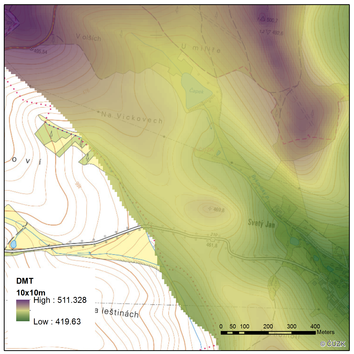
\includegraphics[width=1\linewidth]{./img/DMT_byk.png}
    \caption{\label{fig:dmt}}
  \end{subfigure}%
  \begin{subfigure}[b]{0.4\linewidth}
    \centering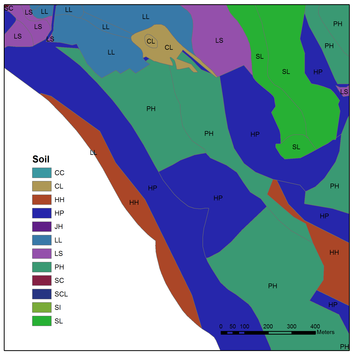
\includegraphics[width=1\linewidth]{./img/pudy.png}
    \caption{\label{fig:puda}}
  \end{subfigure}\\
  \begin{subfigure}[b]{0.4\linewidth}
    \centering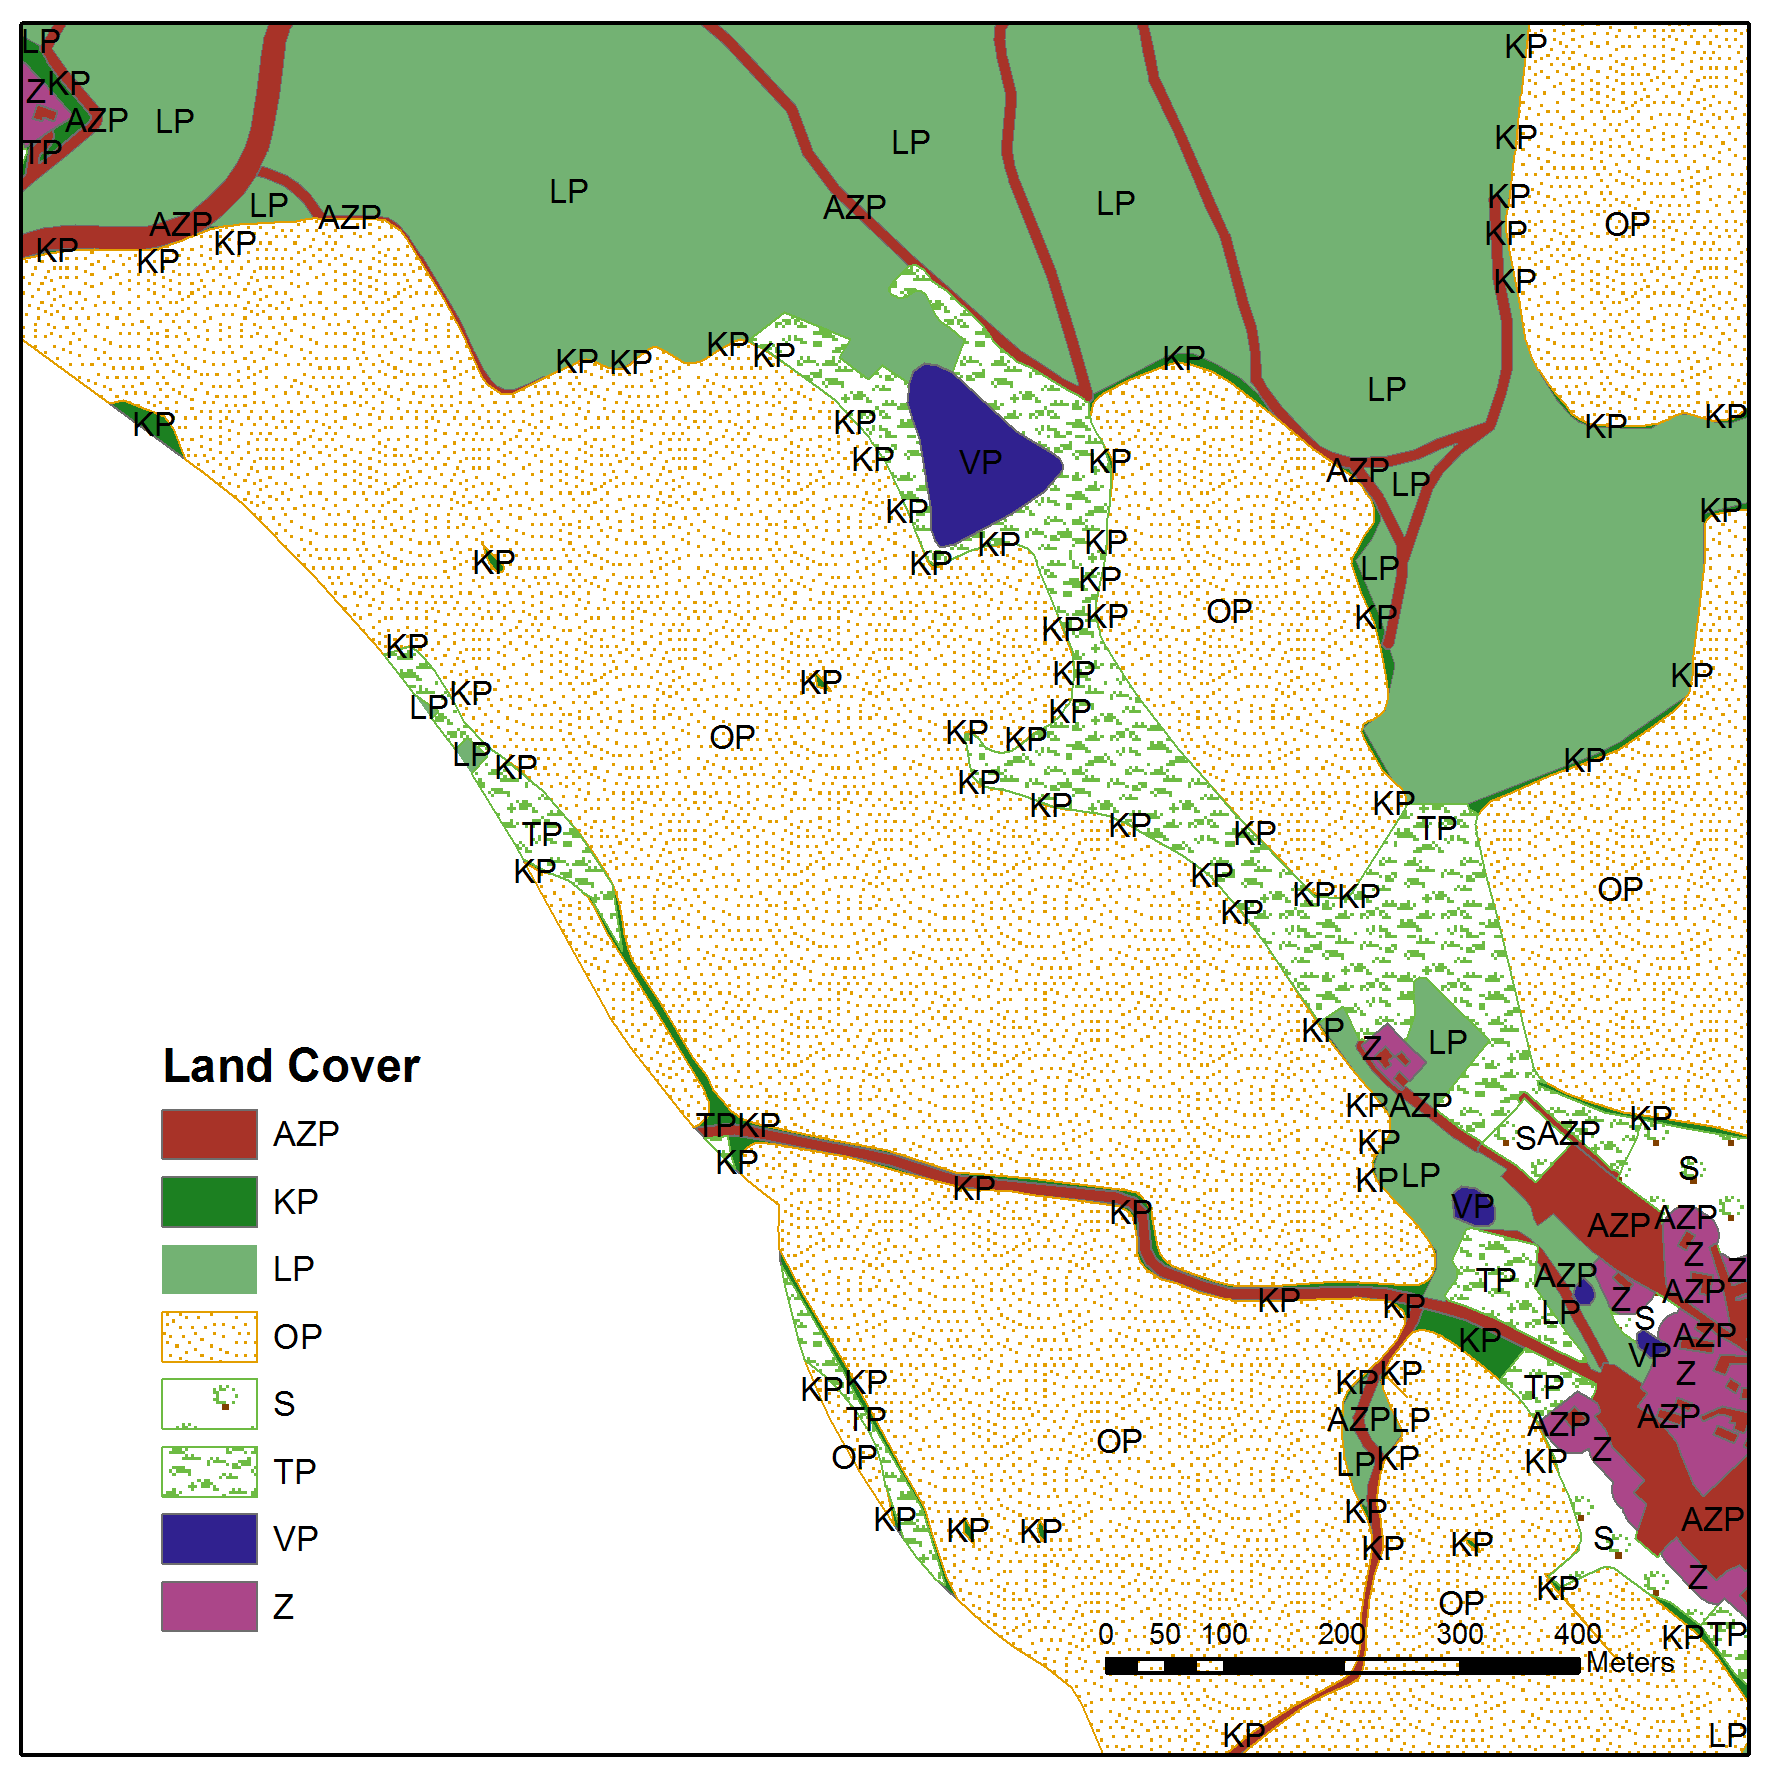
\includegraphics[width=1\linewidth]{./img/LandCover.png}
    \caption{\label{fig:LU}}
  \end{subfigure}%
  \begin{subfigure}[b]{0.4\linewidth}
    \centering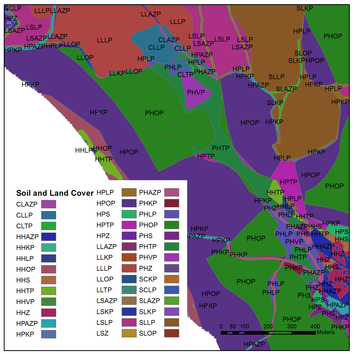
\includegraphics[width=1\linewidth]{./img/SoilAndLC.png}
    \caption{\label{fig:prunik}}
  \end{subfigure}\\
  \begin{subfigure}[b]{0.8\linewidth}
    \centering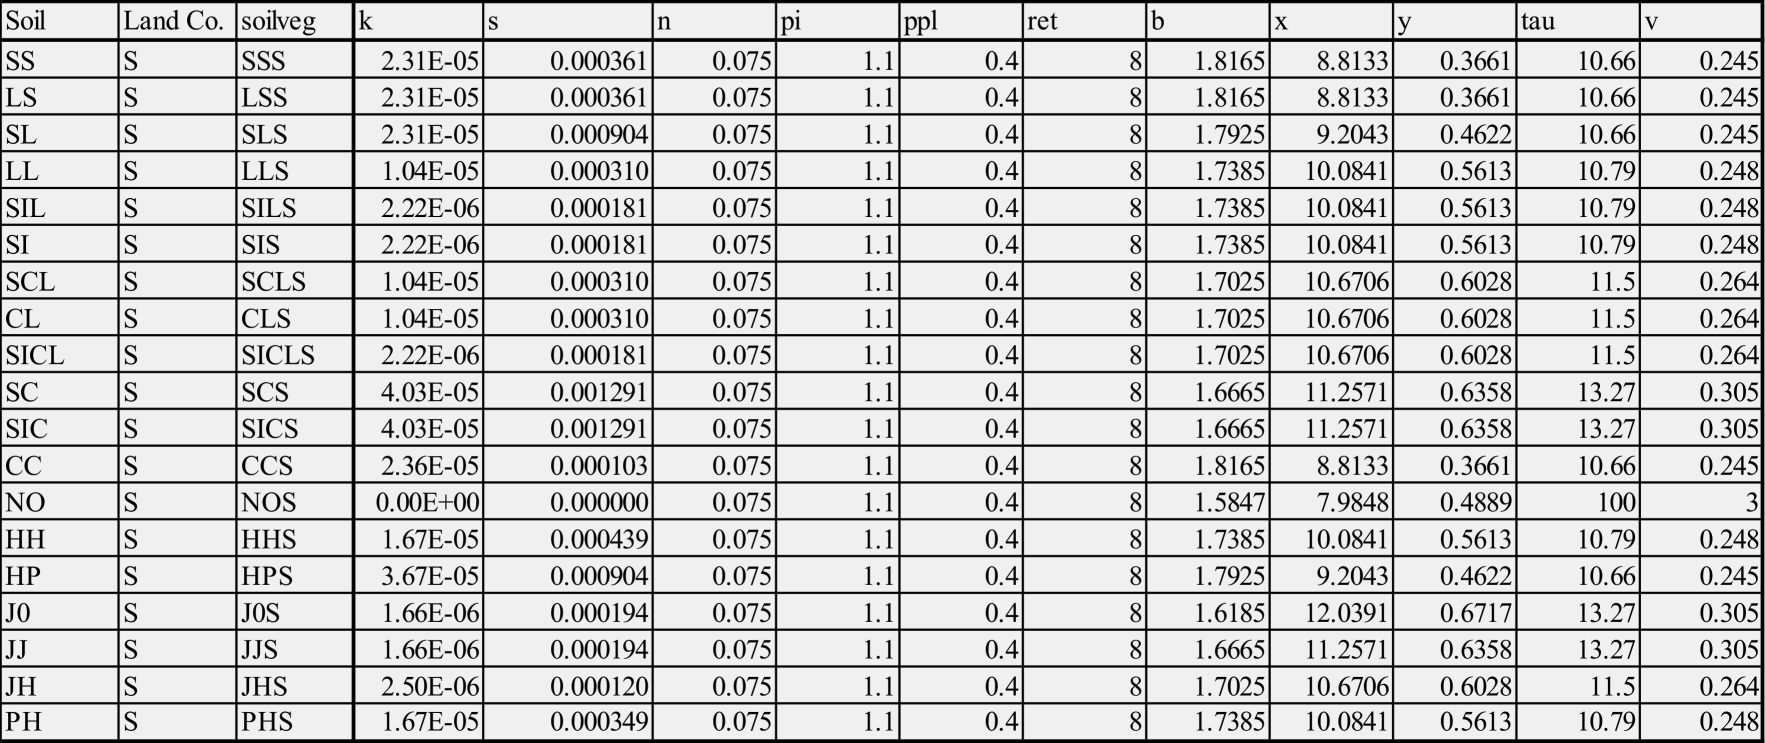
\includegraphics[width=1\linewidth]{./img/soilvegtablo.png}
    \caption{\label{fig:soilvegtablo}}
  \end{subfigure}%
  \caption{Princip propojení vektorových vrstev s tabulkou obsahující parametry typu půd a využití území. Na obrázku a) je digitální model terénu a podkladová mapa. Na obrázku b) je rozložení typu půdy a na obrázku c) rozložení typu využití území. Tyto 2 vrstvy jsou protnuty (funkcí $intersect$). Nové polygony převezmou označení z původních vrstev na obrázku b) a c). Tato nová vektorová vrstva je ukázána na obrázku d). Pomocí převzatých označení polygonů jsou k nim přiřazeny parametry typu půd a využití území z tabulky e).}
  \label{fig:soillu}
\end{figure}



\begin{table}%[!htp]
  \centering
    \caption{Overview of soil type and land use parameters}
    \begin{tabular}{p{3.8cm}l}
    \hline  \hline
        symbol in input table (format mandatory) & description of parameter and unit \\
    \hline
        k&  soil hydraulic conductivity [m/s]\\
        s&  soil sorptivity [$\mathrm{m/s^{1/2}}$]\\
        n&   Mannings surface roughness for sheet flow[-] \\
        b&   power law parameter [-] \\
        y&   power law parameter [-] \\
        nrill&  Mannings surface roughness for rill flow[-] \\
        pi&   potential interception [m]\\
        ppl& canopy cover [-] \\
        ret& surface retention [m] \\
        tau& critical sheer stress [Pa] \\
        v &  critical water velocity [m/s] \\
    \hline  \hline
    \end{tabular}%
  \label{tab:soilveg}%
\end{table}%























\subsection{Srážková data} \label{sec:vstupsrazka}

Dalším vstupem je soubor obsahující srážková data. 
% 
% Na obrázku níže je ukázka textového souboru obsahující proměnlivou srážku, konkrétně je to měření na~rastru Býkovic ze~dne 8.2.2010.
%\begin{figure}[hbt]
%  \centering
 % \includegraphics[scale=1]{obrazky/srazkovysoubor.png}
  %\caption{Srážkový soubor}
%  \label{fig:srazkovysoubor}
%\end{figure}
% 
% 
Srážky se zadávají jako textový soubor se dvěma sloupci. V levém sloupci je časový interval v minutách, v pravém sloupci je \textbf{kumulativní úhrn} za daný časový interval v \textbf{milimetrech}. Ukázka jednoduché srážky a grafické reprezentace kumulativních dat je na obrázku~\ref{fig:srazkovysoubor}. První záznam vyjadřuje srážku od času 0 do například 10 minut (obrázek~\ref{fig:srazkovysoubor}). První záznam v textovém souboru musí mít nenulový čas i úhrn. Soubor může obsahovat prázdné řádky, které jsou ignorovány, nebo komentáře začínající \#. 
\begin{figure}
  \centering
  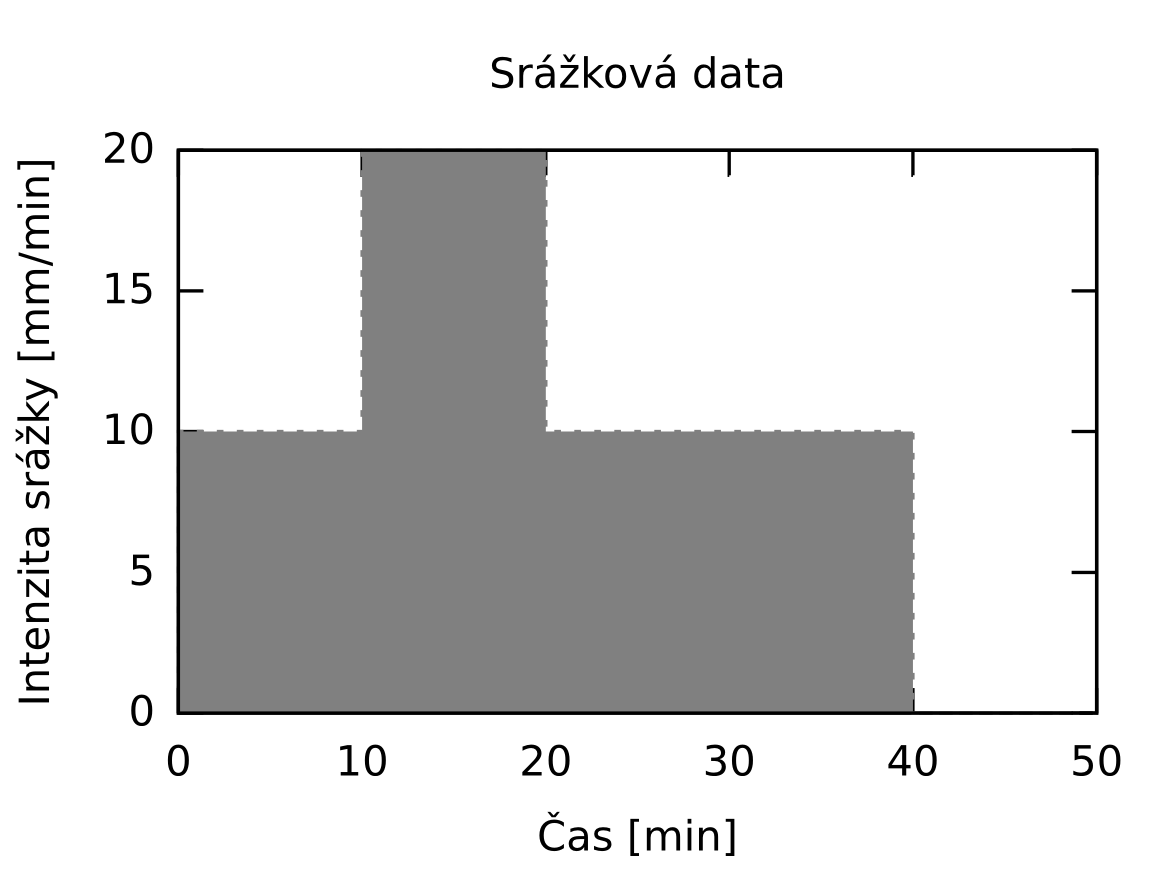
\includegraphics[width=0.45\textwidth]{./img/srazka-graf.png}
  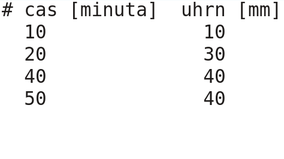
\includegraphics[width=0.5\textwidth]{./img/srazka-soubor.png}
  \caption{Ukázka srážkových dat. Vlevo: grafická reprezentace zadaných dat (srážka zobrazena v intenzitách; Napravo: ukázka dat v požadovaném formátu).}
  \label{fig:srazkovysoubor}
\end{figure}














\subsection{Časový krok modelu a celková doba výpočtu} \label{sec:vstupkrok}

Časový krok modelu \acs{dT} je hodnota v sekundách. Jako vstupní parametr se zadává maximální časový krok. Tento časový krok je rovněž počáteční časový krok. Časový krok \acs{dT} je v průběhu výpočtu upravován podle Courant-Friedrich-Lewy (\acs{CFL}) podmínky tak, aby byla zachována numerická stabilita. Délka časového kroku závisí na rychlosti povrchového odtoku a na velikosti prostorového kroku (velikosti buňky DMT). Maximální časový krok záleží na požadovaném detailu výstupních dat, zejména při dotoku srážkové epizody, kdy jsou již rychlosti proudění nižší a kdy by \acs{CFL} kritérium povolovalo příliš velký časový krok. Zvolené řešení změn časového kroku je detailněji popsáno v kapitole \ref{sec:cfl}. 

%Vzhledem k tomu, že rychlost odtoku v rýhám může být řádově vyšší než rychlost plošného odtoku je snaha řídit velikost časového kroku podle rychlosti plošného odtoku, kde Courantovo kritérium povoluje vyšší časový krok. Velikosti časového kroku zásadně ovlivňuje celkovou délku výpočtu. Pokud časový krok vyhovuje Courantovu kritériu v plošném odtoku, ale toku v rýhách již nikoli, začne se časový krok dělit pouze interně při výpočtu rýh. Tyto děje se probíhají při běhu programu a uživatel je nijak neovlivňuje, nicméně, je třeba si uvědomit, že při vytvoření rýhového odtoku a nutností dělit časový krok v těchto buňkách může se doba výpočtu jednoho časového kroku prodloužit. která udává velikost jednoho kroku výpočtu, v němž probíhá výpočet odtoku a další nedílné součásti programu. Zadaný časový krok se mění podle potřeb Courantova kritéria \ref{section:cfl}, nikdy však nemůže být vyšší než vstupní zadaná hodnota uživatelem. 

%Při zadávání počátečního časového kroku je možno zvolit hodnotu v rozmezí od 0.05 do 0.3 minuty. 
% Velikost časového kroku nejvíce ovlivňuje reálnou dobu běhu modelu. Čím nižší je časový krok, tím déle uživatel čeká na výsledky. 
%Stejně jako u všech ostatních číselných hodnot zadávaných do programu ArcGIS je potřeba myslet na to, že čísla s desetinnými místy musí být odděleny tečkou, nikoliv čárkou.

Konečný čas simulace je hodnota v minutách. Délka běhu modelu by měla být taková, aby odtekla veškerá voda z řešeného území, především při zjišťování celkového objemu odtoku.
 


%\subsection{Povrchová retence} \label{sec:vstupretence}

%Povrchová retence je děj, při kterém se zachytává počáteční část srážky, která se dále neúčastní odtoku. V reálném prostředí si lze toto představit jako zachytávání srážkové vody v nerovnostech na povrchu. Pouze po naplnění těchto malých nerovností dochází k povrchovému odtoku. Hodnota závisí na hustotě půdy a její deformaci. Povrchová retence se zadává v mm. Pro veškerá testování byla povrchová retence zvolena 0.2 mm.













\subsection{Body pro generování hydrogramů} \label{sec:vstupbody}

Jedná  se o volitelnou bodovou vektorovou vrstvu. V těchto bodech se budou ukládat časové řady počítaných veličin (hydrogramy). Obsah časových řad je podrobněji popsán v kapitole~\ref{sec:hydrogramy}.











\subsection{Výstupní adresář} \label{sec:vstupadresar}
Do výstupního adresáře se uloží veškeré výstupy modelu. Na začátku běhu programu se obsah tohoto adresáře celý vymaže, proto se doporučuje vždy provést kontrolu. V žádném případě nenastavujete jako výstupní adresář pracovní plochu, či jiný adresář, kde byste mohli mít uložená důležitá data!

% % % % \subsection{Rýhový odtok} \label{sec:vstupryhovy}
% % % % Tento volitelný parametr po zaškrnutí umožní výpočet soustředěného odtoku. Soustředěný odtok je popsán v sekci \ref{sec:soustredenyodtok}.










% 
% \subsection{Vícesměrný odtok} \label{sec:vstupvicesmerny}
% 
% Výchozí odtokový algoritmus \acl{D8} \acs{D8}. Parametr volby vícesměrného odtokového algoritmu je volitelný. Více o tomto typu odtoku je v části \ref{subsection:MD}
% 
% 
% 







\subsection{Hydrografická síť} \label{sec:vodnitoky}

Hydrografickou sítí jsou myšleny nejen vodní toky, ale i prvky dočasné hydrografické sítě jako jsou příkopy, průlehy, cesty s příkopy a pod. Výpočet v modelu probíhá po jednotlivých úsecích pomocí Manningovy rovnice pro výpočet průtoku (popsané v části~\ref{cast:1}). Prostorové umístění jednotlivých úseků je definované pomocí shapefile liniové vrstvy. Charakteristiky jednotlivých úseků jsou definovány v samostatné tabulce. Pro propojení prostorové informace s charakteristikami úseků je třeba mít v této tabulce shodný název pole jako ve vrstvě vodních toků, kde jsou uloženy označení jednotlivých typů příčných profilů.

V tabulce~\ref{tab:toktab} je ukázka zadávaných hodnot.  Model umožňuje vybrat ze čtyř tvarů příčného průřezu úseků, kde každý tvar má povinné celočíselné označení. Tyto tvary jsou: obdélník (výchozí; tvar: 0), lichoběžník (tvar: 1), trojúhelník (tvar: 2) a parabola (tvar: 3). Kromě tvarových charakteristik (šířka dna, sklon břehu) lze rovněž definovat základní průtok ve formě 365-ti denního průtoku. Pokud úsek charakterizuje objekt, který je pouze dočasně zavodněný, je Q365 = 0. Pole, které slouží k připojení parametrů z tabulky k jednotlivým úsekům hydrografické sítě je v tabulce~\ref{tab:toktab} označeno jako $smoderp$. Rovnice použity při určení hydraulického poloměru jednotlivých tvarů příčných profilů jsou ukázány v tabulce~\ref{fig:tvary_koryt} v příloze~\ref{sec:priloha}.
% 
% Zadávání tvaru příčného profilu není součástí atributové tabulky shapefile, ale pro ulehčení jsou parametry zadávány v samostatná tabulce. V případě, že jsou některé charakteristiky shodné, je tak možné jim přiřadit shodné atributy z tabulky.
% V rámci zjednodušení výpočtu jsou zadávány profily parametricky. Zjednodušený výpočetní model neuvažuje rozlivy z koryta zpět do buněk odtoku. Jednotlivé prvky narůstají podle zvolených parametrů, tak aby veškerá voda zůstala v korytě.
% přehled parametrů je uveden v tabulce~\ref{tab:toptab}

\begin{table}[htb!]
\centering
\caption{Příklad tabulky s parametry jednotlivých úseků hydrografické sítě}
\label{tab:toktab}
\begin{tabular}{llcccccc}
\hline
% 
cislo & smoderp      & tvar & b   & m   & n & Q365 & pozn           \\ \hline \hline
0      & 0            & 1    & 0.3 & 1.0 & 0.03    & 0.0  & default \\
1      & obdelnik1    & 0    & 0.2 & 0.0 & 0.035   & 0.0  &         \\
2      & lichobeznik1 & 1    & 0.2 & 2.0 & 0.035   & 0.0  &         \\
3      & trojuhelnik1 & 2    & 0   & 2.0 & 0.03    & 0.0  &         \\
3      & trojuhelnik2 & 2    & 0   & 2.5 & 0.03    & 15.0  &        \\
4      & parabola1    & 3    & 0.7 & 0.0 & 0.03    & 0.0  &         \\ \hline
\end{tabular}
\end{table}
\FloatBarrier
% 
% 
\begin{tabular}{rrl}
   kde \jj{bhs}{,}
       \jj{m}{,}
       \jj{n}{\ a}
       \jj{Q365}{.}
%        \jj{Rstream}{.}
\end{tabular}

% 
% \pozn{
% kde:
% \begin{itemize}
% \item \textbf{b} - šířka profilu ve dně (u trojúhelníku se rovná nule)
% \item \textbf{m} - poměr sklonu svahů (pro obdélník je roven nule)
% \item \textbf{drsnost} - Maninngova drsnost v daném korytě.
% \item \textbf{Q365} - základní odtok. V případě dočasných prvků jako jsou příkopy je tato hodnota rovna nule, v případě vodních toků se jedná o základní odtok.-
% \item \textbf{poznámky} - jedná se o volitelnou položku, do výpočtu se nijak nepropaguje
% \end{itemize}
% }
% 
% 
% 

 
	
	\section{Popis programu} \label{kap:tok}
	Adresářová struktura programu modelu \smod s popisem nejdůležitějších adresářů a souborů je ukázána na obrázku~\ref{fig:adresare} v příloze~\ref{sec:priloha}. Klíčovým souborem  je  soubor {\tt main.py}, kde se volají dvě základní metody z nichž jedna načte a připraví vstupní data a druhá spustí a provede výpočet.  Dalším důležitým souborem je {\tt src/data\_preparataion.py}, kde probíhá  {\it preprocessing} vstupních dat (v této verzi modelu implementovaný pomocí ArcGIS). Důležitými soubory jsou rovněž soubory {\tt src/runoff.py} a {\tt src/time\_step.py}, kde probíhá samotný výpočet. Soubory v adresáři {\tt src/main\_clasess/} obsahují definici datových struktur jednotlivých řešených dějů a skládají dohromady metody k řešení jednotlivých častí odtoku. Tyto metody jsou pak definované v adresáři {\tt src/processes/}. 

Program \smod je napsaný v jazyce Python. Python je často používaný GIS softwary jako skriptovací jazyk a jsou pro něj k dispozici knihovny pro efektivní práci s geodaty\footnote{knihovna {\tt arcpy} pro ArcGIS či knihovny {\tt grass.script} pro GRASS GIS}. Programy či skripty napsané pomocí Python jsou spustitelné v prostředí daných GIS softwarů. Současná verze modelu \smod používá Python 2.7.X, který je kompatibilní s ArcGIS 10.X.

Na obrázku~\ref{fig:flowchart} v příloze~\ref{sec:priloha} je zjednodušený diagram toku programu. Program řeší v každém časovém kroku rovnici~(\ref{eq:bilancnirce}). Pokud je překročena kritická výška a půda se začne vymílat, začne se do celkového  odtoku  započítávat i soustředěný odtok. Bilanční rovnice je rozšířena (\ref{eq:bilancnircerill}). Pokud je řešen i odtok hydrografickou sítí, načítá se celkový přítok $\sum_j^m \acs{oin}_{j,t-1}$ (případně $\sum_k^n \acs{oinrill}_{k,t-1}$) v rovnici~(\ref{eq:bilancnirce})  nebo (\ref{eq:bilancnircerill}) do všech buněk ležících v daném úseku. Odtok je následně řešen Manningovou rovnicí.

Pokud v daném časovém kroku překročí rychlost v jakékoli buňce \acs{CFL} kritérium, dojde ke zmenšení časového kroku a výpočet se v daném kroku opakuje. Pokud je \acs{CFL} kritérium nízké, je možné časový krok zvýšit. To odpovídá kontrole a aktualizaci časového kroku v diagramu na obrázku~\ref{fig:flowchart}. Po dosažení konečného času dojde k uložení výsledných hodnot a ukončení programu. Pravidla \acs{CFL} kritéria jsou popsána v kapitole~\ref{sec:cfl} a implementována v souboru {\tt src/courant.py}.





% 
% \begin{itemize}
% \item main.py
% \item constants.py
% \item rainfall.py
% \item functions.py
% \item runoff.py
% \item data preparation.py
% \end{itemize}
% 

% \textbf{z diplomky:}
% Samotný model je spouštěn je ze souboru main.py, kde podle zvoleného typu výpočtu je importován příslušný soubor. V současnosti se jedná o soubor runoff.py. Na začátku je provedena příprava dat. Jedná se o soubor data preparation.py. Jádrem přípravných prací je vytvořit ze vstupních dat rozsah řešeného území a vytvořit vrstvu směrů přítoků do jednotlivých buněk. V souboru constants.py jsou označeny vstupy. Soubor functions.py shromažďuje funkce, které se v programu opakují, aby je bylo možno znovu snadněji použít. Soubor rainfall.py převede vstupní textový soubor srážkové události na jednotlivé úhrny podle časového kroku modelu. Samotný výpočet probíhá v jádru souboru runoff.py. Pro jednotlivé časové kroky je vypočítáván povrchový odtok. Výpočet probíhá rozdílně na dvou typech buněk. Plošný odtok je počítán v buňkách, kde hladina nepřekročila hladinu kritickou pro soustředění odtoku a rýhový odtok na buňkách, kde tato hranice překročena byla. Výpočet probíhá ve vícerozměrných maticích. Výsledkem jsou rastry, polygonové vrstvy a textové soubory.




% \textbf{doplnit}
% \begin{itemize}
% \item že se vstupy natahují z AG
% \item časový cyklus
% \item plnění matic a jak je to v matici zapsáno
% \item práce s elementama
% \item co si model pamatuje do dalšího kola
% \item testování výpočtu CLF
% \end{itemize}
% 
% \begin{large}
% \textbf{Někde najité texty}
% \end{large}

% Objektově orientované zpracování toku programu umožňuje jednak lepší orientaci v kódu a také lepší běh programu. Jednotlivé procesy jsou ro







\subsection{Programovací jazyk Python} \label{sec:python}
  Python je vysokoúrovňový objektově orientovaný programovací jazyk, který se může využít v~mnoha oblastech vývoje softwaru. Nabízí významnou podporu k~integraci s~ostatními jazyky a~nástroji a~přichází s~mnoha standardními knihovnami. Jeho použití je velice široké od~programů na~zpracování multimedií až~po~zpracování textů. Python je multiplatformní programovací jazyk~\citep{python}. Zajímavým balíčkem jazyka Pyhton je {\tt numpy}~\citep{numpy}. Je to balíček užívaný pro~vědecké výpočty. Umožňuje manipulaci s velkými multi-dimenzionálními poli a disponuje velkou knihovnou matematických funkcí pro~práci s~těmito poli. Pomocí tohoto balíčku bylo v~programu operováno s~naprostou vetšinou polí a~matic. 
  
  Aktuální verze modelu \smod používá Python 2.7. V~současnosti (Prosinec 2017) je nejnovější verze jazyka Python 3.6. Poslední verze vývojové větve Pythonu 2.7 vyšla v~roce 2010.  Podpora Python 2.7 je plánována do jara 2020 (přesné datum zatím není stanoveno). S koncem podpory Python 2.7 končí i implementace této verze v gis softwarech. ArcGIS PRO již podporuje výhradně Python 3. Proto bude docházek k migraci modelu \smod na verzi  Python~3. 

  
  
  
  
  
  
\subsection{CFL podmínka - řešení nestability výpočtu} \label{sec:cfl}
  V předchozích verzích modelu \smod nebyla ošetřena podmínka stability výpočtu, která vychází z řešení časové derivace. Při větších rychlostech toku či nevhodně zvolené délce časového kroku docházelo k nestabilitám v řešení. Program se v takovém případě ukončil a uložil výsledky posledního úspěšně spočítaného časového kroku. 

  V současné verzi programu \smod je tento problém vyřešen Courant-Friedrich-Lewy (\acs{CFL}) podmínkou. Splnění této podmínky zajišťuje konvergenci explicitního řešení pokud platí, že $\acs{CFL} < 1.0$. Z obecné rovnice \acs{CFL} podmínky byla odvozena a upravena podmínka pro účely modelu \smod na následující tvar: \pozn{neni k tomu 0.5601 nejak citace?} 
  \begin{equation}
    \acs{CFL} = \frac{1}{0.5601}\frac{v \acs{dT}}{\acs{dX}} 
    \label{eq:courrovnice}
  \end{equation}
  \begin{tabular}{rrl}
    kde \jj{CFL}{,}
        & $v$ & je rychlost plošného či rýhového toku [$m/s$], \\
        \jj{dT}{\ a}
        \jj{dX}{.}
  \end{tabular}
  
  Po dokončení výpočtu  časového kroku je uložena nejvyšší hodnota \acs{CFL} zjištěná z {\bf plošného odtoku} pomocí vztahu~(\ref{eq:courrovnice}). Poté se tato hodnota porovná s kritickou hodnotou \acs{CFL} a podle pravidel znázorněných v tabulce~\ref{tab:cflsheet} se změní (nebo nezmění) délka časového kroku \acs{dT}. Pokud dojde ke změně \acs{dT} opakuje se výpočet v daném časovém kroku a aktualizovaným \acs{dT}. Do dalšího času se výpočet posune, až když je zaručena stabilita výpočtu. 
  
  \begin{table}[t!]
    \centering
    \caption{Kritéria změny časového kroku vycházející z plošného odtoku}
    \label{tab:cflsheet}
    \begin{tabular}{ccc}
      \hline
        nové  &  $\acs{CFL} < 0.75 \lor 1.0 < \acs{CFL}$ & $ 0.75 \geq \acs{CFL} \geq 1.0 \lor \acs{CFL} = 0.0^*$ \\
        \hline
        \hline
        \acs{dT} &  = $MIN(\frac{0.5601\acs{dX}}{v};\acs{dTmax})$ & = původní \acs{dT}\\
        \hline
%         \multicolumn{3}{l}{{\small \acs{CFL} = 0.0 zpravidla v případně, pokud je rychlost proudění nulová. Potom nelze }}
    \end{tabular}
  \end{table}

  {\bf Soustředěný odtok} v  rýhách je zpravidla řádově rychlejší než plošný odtok. Pokud bychom v tomto případě uplatňovali stejný princip jako u plošného odtoku, časový krok by byl extrémně malý, čímž by se prodlužoval strojový čas výpočtu. K odtoku v rýhách většinou nedochází na celém území, ale pouze v poměrně malém počtu buněk (v poměru k celé ploše výpočetní oblasti). Proto se při výpočtu soustředěného odtoku přistoupilo k lokálnímu krácení časového kroku pouze v buňkách, kde k soustředěnému odtoku dojde. Časový krok výpočtu odtoku v rýhách je dělen celočíselně faktorem označeným jako \acs{ratio}.  \acs{CFL} číslo se proto ukládá zvlášť u plošného a zvlášť u soustředěného odtoku. Ke změně celkového časového kroku plošného odtoku dojde až pokud $\acs{ratio} >= 10$. Časový krok plošného odtoku je pak násoben multiplikátorem \acs{dTmult}, který se po každém překročení kritické \acs{CFL} podmínky zmenší na 90 \% své dosavadní hodnoty. Pokud je \acs{CFL} kritérium příznivé (začíná se zmenšovat), multiplikátor \acs{dTmult} se postupně zvětšuje vždy o 10 \% dokud nedosáhne hodnoty 1. Pravidla pro změna faktoru \acs{ratio} a multiplikátoru \acs{dTmult} jsou shrnuta tabulce~\ref{tab:cflrill}.
  \begin{table}[t!]
    \centering
    \caption{Kritéria změny faktoru \acs{ratio} při dělení časového kroku pří výpočtu rýhového odtoku}
    \label{tab:cflrill}
    {\small
    \begin{tabular}{llll}
      \hline
        nové  &  $\acs{CFL}_{rill} < 0.3 $ & $ 0.5 < \acs{CFL}_{rill}$ & $ 0.3 \geq \acs{CFL}_{rill} \geq 0.5 $ \\
        & & & $\lor \acs{CFL}_{rill} = 0.0 $ \\
        \hline
        \hline
        \acs{ratio} &  = $MAX(\acs{ratio} - 1;1)$ &  = $MIN(\acs{ratio} + 1;9)$ & = původní \acs{ratio}\\
                     &                              &  pro \acs{ratio} = 10  &                            \\
        \acs{dTmult} &  = $MIN((1/0.9)\acs{dTmult};1)$ &  = $0.9\acs{dTmult}$ & = původní \acs{dTmult}\\
        \acs{dT}    &  & \multicolumn{2}{l}{= $\acs{dT}\acs{dTmult}$} \\
        \hline
        
    \end{tabular}
    }
  \end{table}
  
  
  Obrázek \ref{fig:cfl1} a \ref{fig:cfl2} ukazují chování časového kroku v případě, že je řízen plošným (obrázek~\ref{fig:cfl1}) nebo soustředěným odtokem (obrázek~\ref{fig:cfl2}). 
%   
%   
  \begin{figure}[p]
    \centering
    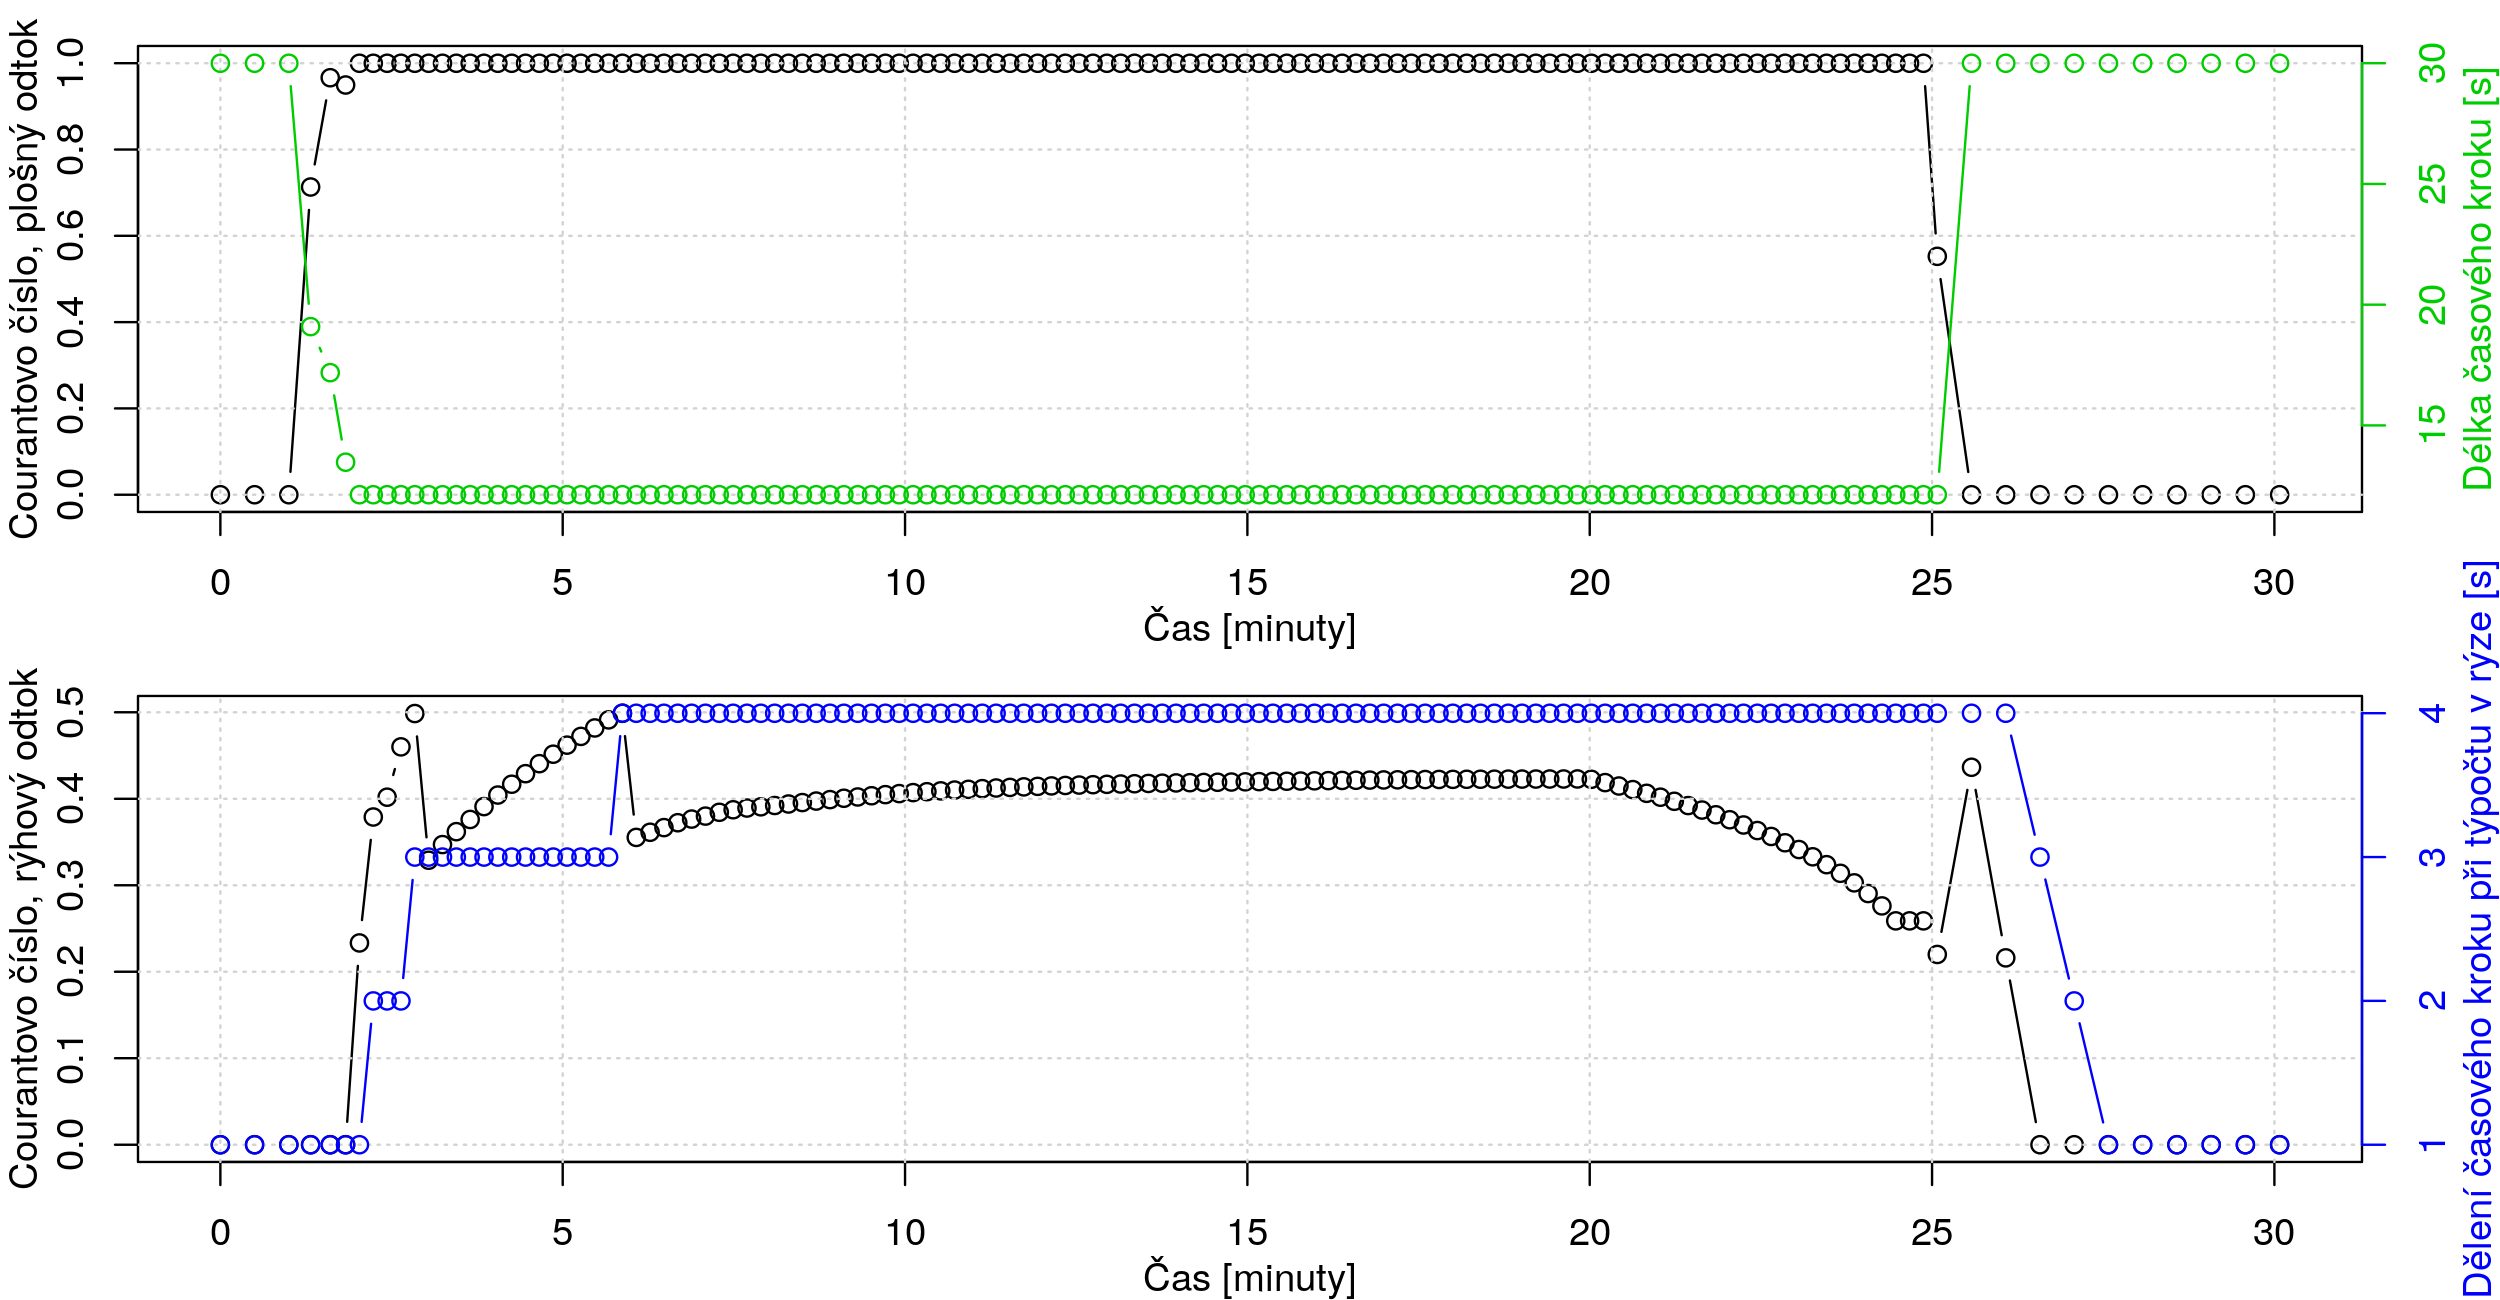
\includegraphics[width=0.8\textwidth]{./img/courantratio.png}
    \caption{Časový krok je řízen rychlostí plošného odtoku. \acs{CFL} rychle stoupne k 1 a začne zkracovat časový krok (horní graf). O pár minut později $\acs{CFL}_{rill}$ stoupne nad 0.5, \acs{ratio} stoupne na 2 (dolní graf) tím začne lokálně dělit časový krok při výpočtu rýhového odtoku. \acs{ratio} na spodním grafu stoupne maximálně na 4 a neovlivní tedy celkový časový krok (na horním grafu). Na obou grafech je vidět, jak se po 25. minutě (kdy v modelu skončila srážková událost) délka časového kroku i \acs{ratio} vrátí na původní hodnoty.}
    \label{fig:cfl1}
  \end{figure}
%   
%   
  \begin{figure}[p]
    \centering
    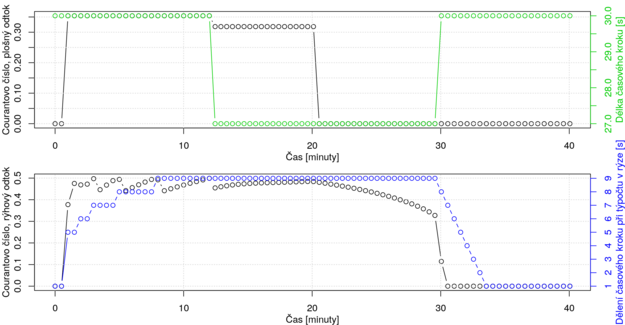
\includegraphics[width=0.8\textwidth]{./img/courantratio2.png}
    \caption{Časový krok je řízen rychlostí rýhového odtoku.  \acs{CFL} plošného odtoku nepřekročí během výpočtu hodnotu cca 0.35 (na horním grafu), proto nemá žádný vliv na velikost časového kroku.  $\acs{CFL}_{rill}$ rychle vystoupí 9 krát nad kritickou hodnotu 0.5 (spodní graf, prvních 10 minut výpočtu). To způsobí nárůst \acs{ratio} na 9, což je maximální povolené dělení lokálního časového kroku při výpočtu rýhového odtoku. Pří dalším překročení hodnot 0.3 (cca 12. minuta na dolním grafu) dojde ke zmenšení celkového časového kroku na 90 \% původní hodnoty (horní graf). Na obou grafech je vidět jak se po 20. minutě (kdy v modelu skončila srážková událost) délka časového kroku i \acs{ratio} vrátí na původní hodnoty.}
    \label{fig:cfl2}
  \end{figure}
  

% Hlavní myšlenkou řešení nestability výpočtu je zmenšení časového kroku při náznaku, že by mohlo dojít k přetečení. Pro každý časový krok je podle rovnice \ref{courrovnice} vypočteno v každé buňce Courantovo číslo $C$. Dále je určeno maximum Courantova čísla ve všech buňkách v časovém kroku. Toto číslo je zásádní, jelikož podle něj se porovnává, zda je situace potencionálně nebezpečná a bude potřeba zmenšit časový krok. Na změnu časového kroku byla použita funkce pojmenovaná $courant$:

% Dochází k porovnání, zda se Courant pohybuje v rozmezí hodnot 0.8 a 1.0. Pokud je hodnota vyšší, je zmenšen časový krok  a pokud je hodnota nižší, časový krok se zvýší. Nikdy však nemůže být výšší než původní časový krok zadaný. Testování probíhalo tak, aby podmínka zmenšila co možná nejméně časový krok a při tom nedošlo k numerické nestabilitě v kroku následujícím. Velikost časového kroku $\Delta t$ zásadně ovlivňuje dobu běhu celého modelu. Čím více se zmenší časový krok, tím déle trvá modelu než doběhne do požadové časové hodnoty a ukončí se. V současné verzi je největším problémem fakt, že při větších průtocích na větším území dojde brzy ke zmenšení $\Delta t$ na velmi nízkou hodnotu, např. 0.01 minuty a tím se úměrně zvyšuje časová náročnost výpočtů.





	
	\newpage
	\section{Výstupy z modelu} \label{kap:vystupy}
	
\pozn{
\textbf{Zde dodelat}
\begin{itemize}
  \item popsat výstupy mimo temp
  \item popsat co jsou v temp
  \item popsat výstupy v určitých krocích
\end{itemize}
}


Výstupy modelu jsou uloženy do složky zadané mezi vstupními parametry (obsah složky je při spuštění programu vymazán!). Kumulativní nebo maximální hodnoty veličin v jednotlivých  buňkách jsou na konci výpočtu uloženy v rastrovém formátu (viz kapitola~\ref{sec:rastr}). Průnik polygonů prostorové distribuce typu půd a využití území jsou uloženy ve vektorovém formátu (viz kapitola~\ref{sec:vektor}). Pokud model \smod počítá i úseky hydrografické sítě, jsou kumulativní nebo maximální hodnoty veličin jednotlivých úseků vypsáný v atributové tabulce vektorové vrstvy úseků (viz kapitola~\ref{sec:vektor}). Prostorové rozložení jednotlivých úseků je uloženo také jako jeden s rastrů (viz kapitola~\ref{sec:rastr}).  Volitelné výstupy hydrogramů  v bodech jsou ve formě časových řad uloženy do textových souborů s příponou {\tt.dat} (viz kapitola~\ref{sec:hydrogramy}). Další nadstandardní výstupy lze získat způsobem popsaným v příloze~\ref{sec:priloha2}. Jednotlivé výstupy jsou dále popsány podrobněji. 













\subsection{Rastrové výstupy}\label{sec:rastr}

V rastrech jsou uloženy maximální a kumulativní hodnoty vybraných veličin v jednotlivých buňkách řešeného území. Jako rastrový formát lze zvolit proprietární ESRI formát nebo textový formát ASII. Přehled rastrových výstupních souborů je shrnut v tabulce~\ref{tab:vystupyrast}. Pokud jsou v modelu řešeny i úseky hydrografické sítě, jsou buňky rastru ležící na úseku uloženy s hodnotou {\tt NoData} (výjimku tvoří 2 rastry popisující vlastnosti úseků, viz tabulka~\ref{tab:vystupyrast}).  


% jsou ve textovém nebo rastrovém formátu.  








\subsection{Vektorové výstupy}\label{sec:vektor}

Výstupní vektorová data jsou tři. Jedná se topologicky upravenou vrstvu úseků hydrografické sítě ({\tt hydReach}), kde jsou do její atributové tabulky doplněny kumulativní a maximální hodnoty vybraných veličin. Tyto veličiny jsou popsány v tabulce~\ref{tab:useky}. Druhým vektorovým výstupem je vrstva, která zobrazuje průnik prostorového rozložení typu půdy a využití území ({\tt interSoilLU}). Ukázka takové vrstvy je na obrázku~\ref{fig:soillu}. Tato vektorová vrstva slouží především ke kontrole správnosti přípravy vstupních dat či hledání chyb v nich. Při $preprocessingu$ jsou  z (nepovinné) bodové vrstvy pro zápis hydrogramů smazány body, které jsou mimo výpočetní oblast. Proto je ve výsledcích uložena vrstva s body, které jsou skutečné pro výpis hydrogramů použity. Tato bodová vrstva má název {\tt pointsCheck}. 













\subsection{Hydrogramy}\label{sec:hydrogramy}

Pokud jsou do vstupů zadány body pro výpis hydrogramů, vypíší se do textových souborů s příponou {\tt.dat}. Vypsané veličiny jsou závislé na typu odtokového procesu. Popis vypsaných veličin  povrchového odtoku je v tabulce~\ref{tab:vystupydat}. Pokud je bod v buňce úseku hydrografické sítě, vypisují se hodnoty tohoto celého úseku, přestože tento bod není na konci úseku.  Názvy a význam veličin popisujících úsek toku jsou popsány v tabulce~\ref{tab:vystupytokdat}.  Model v současné verzi uvažuje, že pokud je v buňce úsek hydrografické sítě, zabírá úsek celou buňku, přestože je jeho šířka menší než šířka samotné buňky.  Název těchto souborů je odvozen z FID upravené bodové vrstvy {\tt pointsCheck} ve tvaru $point$\{{\tt pointsCheck}:FID\}$.dat$. 





% 11.12. Zakomentova radky jsou to tempu


\begin{table}[t]
 

 \centering
 \caption{Přehled rastrových výstupů}
\label{tab:vystupyrast}

% \begin{tabular}{p{4cm}lp{2cm}p{5cm}}
 \begin{tabular}{llp{0.5\textwidth}}
 \hline \hline
  Název souboru    & Jednotka    & Popis       \\ 
  (ESRI nebo .acs)    &     &        \\ \hline 
  cinfilt\_m      &   $m$        & Kumulativní infiltrace \\
  crainf\_m          &  $m$    &  Kumulativní srážka (bez intercepce a povrchové retence) \\
%   csheetvout\_m3      &  $m^3$  & Kumulativní objem odtoku z buňky \\
%   crillvout\_m3       &  $m^3$  & Kumulativní objem odtoku z buňky rýhou \\
  csurvout\_m3       &  $m^3$  & Kumulativní objem odtoku z buňky \\
%   cvin\_m3            &  $m^3$  & Kumulativní objem přítoků do buňky  (plošný + soustředěný) \\
  volrest\_m3          &  $m^3$  & Objem vody zbylé v buňkách po zkončení výpočtu\\
  dmt                 &  $m$ &  Výřez použitého digitálního modelu terénu \\
  flowdir             &  $NA$ &  Rastr s uloženými směry odtoku  \\
  mshearstr\_pa      & $Pa$ &  Maximální tečné napětí \\
%   mreachflm3\_s     &  $m^3s^{-1}$ & Maximální odtok v úsecích hyd. sítě  \\
  msurfl\_m3\_s   &   $m^3s^{-1}$ &  Maximální celkový odtok v buňce\\
  mvel\_m\_s       &   $ms^{-1}$ &  Maximální rychlost proudění v buňce (plošného či soustředěného odtoku) \\
  reachFID            &  $NA$  &  Označuje úseky toku (=fid + 1000), buňky s plošným odtokem (=0) a plošným i soustředěným odtokem (=1) \\
  massbalance         &   $m$  &  Bilance všech vstupů a výstupu z a do buňky  \\
  \hline \hline
%  tyhle jdou do tempu
%  rillAreaM       &   $m^2$      &  Plocha buňky, kterou porývá rýha \\
%  finalCellState    &  $NA$ & Typ odtoku buňky na konci výpočtu (viz sekce~\ref{sec:statpopis})\\
%  critWaterLevelM         & $m$    &  kritický výška hladiny \\
%  mSheetFlowM3_S	  &   $m^3-s^{-1}$	&  Maximální plošný průtok v buňce  \\
%  mRillFlowM3_S    &   $m^3-s^{-1}$	&  Maximální soustředěný průtok v buňce\\
%  mSheetWaterLevelM    &   $m$  &   Maximální výška hladiny plošného v buňce \\
%  mRillWaterLevelM   &   $m$  &   Maximální výška hladiny soustředěného odtoku v buňce \\

 \end{tabular}
 

\end{table}


% cInfiltrationM
% cRainfallM
% cSheetVolOutM3 
% cRillVolOutM3
% cSurfaceVolOutM3
% cVolRestM3
% cReachVolOutM3
% mSurfaceFlowM3_S
% mVelocityM_S
% mReachFlowM3_S
% mShearStressPa
% reachFID
% massBalance





% zakomentovane je do tmp




\begin{table}[t]
 

 \centering
 \caption{Popis veličin  tabulky úseků hydrografické sítě}
\label{tab:useky}

% \begin{tabular}{p{4cm}lp{2cm}p{5cm}}
 \begin{tabular}{llp{0.5\textwidth}}
  \hline  \hline
 Název sloupce        & Jednotka     & Popis                                 \\ 
 \hline
 FID            &   ---          &  Identifikátor přiřazeného úseku ({\it feature id})   \\
 cVolM3         &  $m^3$         & Kumulativní objem odtoku                              \\
 mFlowM3\_S      &   $m^3s_{-1}$  & Maximální průtok                                      \\
 mFlowTimeS     &   $s$          &  Čas dosažení maximálního průtoku                     \\
 mWatLM         &  $m$       &  Maximální výška hladiny v úseku                               \\
%  mWatLTimeS     &  $s$       &  Čas dosažení maximálního průtoku                              \\
%  cSurInFM3      &  $m^3$     &  Kumulativní přítok do úseku z jeho okolí   \\
 restVolM3      &  $m^3$     &  Objem v úseku po skončení výpočtu         \\
%  cVolDomM3      &  $m^3$     &  Kumulativní odtok úseku z řešeného území (hodnota je nulová pokud úsek odtéká do jiného navazujícího úseku)   \\
 toFID          &  ---       &  FID úseku do které daný úsek odtéká (hodnota -9999 vyjadřuje situaci, kdy úsek kříží hranici řešeného a odtéká tedy mimo toto území) \\
  \hline
   \hline
 \end{tabular}

\end{table}



% FID;V_out_cum [L^3];Q_max [L^3.t^{-1}];timeQ_max[s];h_max [L];timeh_max[s];
% Cumulatice_inflow_from_field[L^3];Left_after_last_time_step[L^3];Out_form_domain[L^3];to_reach



% % zakomentovane je do tmp

\begin{table}[t]
 

 \centering
 \caption{Popis veličin hydrogramů mimo úsek hydrografické sítě}
\label{tab:vystupydat}

% \begin{tabular}{p{4cm}lp{2cm}p{5cm}}
 \begin{tabular}{llp{0.5\textwidth}}
  \hline  \hline
 Název sloupce    & Jednotka    & Popis       \\ 
  \hline
%  \hline
%  Buňka s plošným odtokem:	 &&\\
 time[s]          &   $s$      &  Čas od začátku simulace          \\
 deltaTime[s]     &   $s$        &  Aktuální délka časového kroku  \\
 rainfall[m]      &  $m$         &  Srážková výška v aktuálním časovém kroku \\
%  sheetWaterLevel[m]       &  $m^3$  & Výška hladiny plošného odtoku \\
%  sheetFlow[m3/s]       &  $m^3s^{-1}$  & Průtok plošného odtoku  \\
%  sheetVolRunoff[m3]    &  $m^3$     & Odteklý objem plošného odtoku \\
%  sheetVolRest[m3]      &  $m^3$     & Objem zbytku vody po plošném odtoku \\
%  infiltration[m]         &  $m$      & Výška infiltrace v daném časovém kroku \\
%  surfaceRetention[m]    &  $m$      & Výška zadržené vody na povrchu v daném časovém kroku \\
%  callState                   &  -         & Typ odtoku na buňce (viz sekce~\ref{sec:statpopis})  \\
%  inflowVol[m3]   &   $m^3$ &  Celkový objem přítoku do buňky \\
 totalWaterLevel[m]$^*$	  &   $m$	&  Celková výška hladiny  \\ 
%  \hline
%  Pro soustředěný odtok &&\\ \hline 
%  rillWaterLevel[m]         &   $m$       &  Výška hladiny v buňce se soustředěným odtokem* \\
%  rillWidth[m]	       &   $m$ &  Šířka rýhy vzniklá soustředěným odtokem\\
%  rillFlow[m3/s]      &   $m^3s^{-1}$       &  Průtok v rýze soustředěného odtoku \\
%  rillVolRunoff[m3]   &   $m^3$  &   Objem soustředěného odtoku rýhou \\
%  rillVolRest[m3]  &  $m^3$ &   Objem zbytku vody po soustředěném odtoku rýhou  \\
 surfaceFlow[m3/s]   &  $m^3_{-1}$ & Celkový průtok (plošný + soustředěný)  \\
 surfaceVolRunoff[m3]   &   $m$  & Celkový odteklý objem (plošný + soustředěný) \\
%  rillInflowVol[m3] & $m$ &  @@@ toto tam chcem? to je V\_inflow cast co jde do ryhy, pridal jsem to tam jednou kdyz jsem hledal nejakou chybu...\\
%  ratio & $m$ &  Počet krácení časového kroku v rýhách @@@(je pro nas?)\\
%  sheetCourantCrit & $m$ &  Courantovo kritérium pro plošná odtok @@@(je pro nas?)\\
%  rillCourantCrit & $m$ & Courantovo kritérium pro soustředěný odtok @@@(je pro nas?) \\
%  nIter & $m$ &  Počet iterací pří výpočty daného výpočetního kroku @@@(to bych tam nechal, muže to napověděl jestli se tam neděje něco moc rychle, což může znamenat chybu v zadaných datech, třeba dát 600 mm do srážky místo 60 mm) \\
  \hline
   \hline
   \multicolumn{3}{p{\textwidth}}{*výška hladiny u soustředěného odtoku není skutečná výška hladiny v rýze, ale nadkritická výška hladiny vztažená na celou plochu výpočetní buňky}
 \end{tabular}

\end{table}

% zakomentovane je do tmp

\begin{table}[t]
 

 \centering
 \caption{Popis veličin hydrogramů mimo úsek hydrografické sítě}
\label{tab:vystupydat}

% \begin{tabular}{p{4cm}lp{2cm}p{5cm}}
 \begin{tabular}{llp{0.5\textwidth}}
  \hline  \hline
 Název sloupce    & Jednotka    & Popis       \\ 
  \hline
%  \hline
%  Buňka s plošným odtokem:	 &&\\
 time[s]          &   $s$      &  Čas od začátku simulace          \\
 deltaTime[s]     &   $s$        &  Aktuální délka časového kroku  \\
 rainfall[m]      &  $m$         &  Srážková výška v aktuálním časovém kroku \\
%  sheetWaterLevel[m]       &  $m^3$  & Výška hladiny plošného odtoku \\
%  sheetFlow[m3/s]       &  $m^3s^{-1}$  & Průtok plošného odtoku  \\
%  sheetVolRunoff[m3]    &  $m^3$     & Odteklý objem plošného odtoku \\
%  sheetVolRest[m3]      &  $m^3$     & Objem zbytku vody po plošném odtoku \\
%  infiltration[m]         &  $m$      & Výška infiltrace v daném časovém kroku \\
%  surfaceRetention[m]    &  $m$      & Výška zadržené vody na povrchu v daném časovém kroku \\
%  callState                   &  -         & Typ odtoku na buňce (viz sekce~\ref{sec:statpopis})  \\
%  inflowVol[m3]   &   $m^3$ &  Celkový objem přítoku do buňky \\
 totalWaterLevel[m]$^*$	  &   $m$	&  Celková výška hladiny  \\ 
%  \hline
%  Pro soustředěný odtok &&\\ \hline 
%  rillWaterLevel[m]         &   $m$       &  Výška hladiny v buňce se soustředěným odtokem* \\
%  rillWidth[m]	       &   $m$ &  Šířka rýhy vzniklá soustředěným odtokem\\
%  rillFlow[m3/s]      &   $m^3s^{-1}$       &  Průtok v rýze soustředěného odtoku \\
%  rillVolRunoff[m3]   &   $m^3$  &   Objem soustředěného odtoku rýhou \\
%  rillVolRest[m3]  &  $m^3$ &   Objem zbytku vody po soustředěném odtoku rýhou  \\
 surfaceFlow[m3/s]   &  $m^3_{-1}$ & Celkový průtok (plošný + soustředěný)  \\
 surfaceVolRunoff[m3]   &   $m$  & Celkový odteklý objem (plošný + soustředěný) \\
%  rillInflowVol[m3] & $m$ &  @@@ toto tam chcem? to je V\_inflow cast co jde do ryhy, pridal jsem to tam jednou kdyz jsem hledal nejakou chybu...\\
%  ratio & $m$ &  Počet krácení časového kroku v rýhách @@@(je pro nas?)\\
%  sheetCourantCrit & $m$ &  Courantovo kritérium pro plošná odtok @@@(je pro nas?)\\
%  rillCourantCrit & $m$ & Courantovo kritérium pro soustředěný odtok @@@(je pro nas?) \\
%  nIter & $m$ &  Počet iterací pří výpočty daného výpočetního kroku @@@(to bych tam nechal, muže to napověděl jestli se tam neděje něco moc rychle, což může znamenat chybu v zadaných datech, třeba dát 600 mm do srážky místo 60 mm) \\
  \hline
   \hline
   \multicolumn{3}{p{\textwidth}}{*výška hladiny u soustředěného odtoku není skutečná výška hladiny v rýze, ale nadkritická výška hladiny vztažená na celou plochu výpočetní buňky}
 \end{tabular}

\end{table}


% % zakomentovane je do tmp



\begin{table}[t]
 

 \centering
 \caption{Popis veličin  hydrogramů v úsecích hydrografické sítě}
\label{tab:vystupytokdat}

% \begin{tabular}{p{4cm}lp{2cm}p{5cm}}
 \begin{tabular}{llp{0.5\textwidth}}
  \hline  \hline
 Název sloupce        & Jednotka     & Popis                                      \\ 
 \hline
 time[s]              &   $s$              &  Čas od začátku simulace                   \\
 deltaTime[s]         &   $s$              &  Aktuální délka časového kroku            \\
 rainfall[m]          &  $m$               &  Srážková výška v aktuálním časovém kroku \\
 reachWaterLevel[m]        &  $m$          &  Výška hladiny plošného odtoku            \\
 reachFlow[m3/s]              &  $m^3s^{-1}$   &  Průtok plošného odtoku                   \\
 reachVolRunoff[m3]           &  $m^3$         & Odteklý objem plošného odtoku     \\
%  reachVolInflow[m3]              &  $m^3$     & Suma přítoků z okolních buněk úseku v daném časovém kroku \\
%  reachVolRest[m3]         &  $m^3$     & Objem v úseku toku po odtoku      \\
  \hline  \hline
 \end{tabular}

\end{table}

% # Time[s];deltaTime[s];Rainfall[m];Waterlevel[m];V_runoff[m3];Q[m3/s];V_from_field[m3];V_rests_in_stream[m3]
% 
% 
% time[s]
% deltaTime[s]
% rainfall[m]
% reachWaterLevel[m]
% reachFlow[m3/s]
% reachVolRunoff[m3/s]
% reachVolInflow[m3]
% reachVolRest[m]
% zakomentovane je do tmp



\begin{table}[t]
 

 \centering
 \caption{Popis veličin  hydrogramů v úsecích hydrografické sítě}
\label{tab:vystupytokdat}

% \begin{tabular}{p{4cm}lp{2cm}p{5cm}}
 \begin{tabular}{llp{0.5\textwidth}}
  \hline  \hline
 Název sloupce        & Jednotka     & Popis                                      \\ 
 \hline
 time[s]              &   $s$              &  Čas od začátku simulace                   \\
 deltaTime[s]         &   $s$              &  Aktuální délka časového kroku            \\
 rainfall[m]          &  $m$               &  Srážková výška v aktuálním časovém kroku \\
 reachWaterLevel[m]        &  $m$          &  Výška hladiny plošného odtoku            \\
 reachFlow[m3/s]              &  $m^3s^{-1}$   &  Průtok plošného odtoku                   \\
 reachVolRunoff[m3]           &  $m^3$         & Odteklý objem plošného odtoku     \\
%  reachVolInflow[m3]              &  $m^3$     & Suma přítoků z okolních buněk úseku v daném časovém kroku \\
%  reachVolRest[m3]         &  $m^3$     & Objem v úseku toku po odtoku      \\
  \hline  \hline
 \end{tabular}

\end{table}

% # Time[s];deltaTime[s];Rainfall[m];Waterlevel[m];V_runoff[m3];Q[m3/s];V_from_field[m3];V_rests_in_stream[m3]
% 
% 
% time[s]
% deltaTime[s]
% rainfall[m]
% reachWaterLevel[m]
% reachFlow[m3/s]
% reachVolRunoff[m3/s]
% reachVolInflow[m3]
% reachVolRest[m]











% \subsection{State - typ průtoku na buňce}\label{sec:statpopis}
%   Jak bylo popsání no v kapitole~\ref{kap:tok} v modelu je možné řešit několik typů povrchového odtoku: plošný odtok, soustředěný odtoku a odtok hydrografickou sítí. Topografie hydrografické sítě je definována uživatelem. Vznik soustředěného odtoku je podmíněn překročením kritické výšky (popsáno v kapitole~\ref{sec:soustredenyodtok}). V programu jsou typy odtoku rozlišeny celočíselným identifikátorem označeným State, kde pokud State\\
% %   
%   \begin{tabular}{rcl}
%      =     &0&  dochází v buňce pouze k plošnému odtoku pokud \\
%      =     &1&  dochází v buňce k plošnému i soustředěnému odtoku  nebo pokud \\
%      =     &2&  @@@ plošný odtoku a rýha jen odtéká \\
%      && je to v teto verzi? Je to zajímavé pro uživatele? \\
%      $>$=  &1000&  je v buňce úsek hydrografické sítě. \\
%   \end{tabular}
% 
%   Identifikátor hydrografické sítě nemusí začínat číslem 1000 a nemusí být vzestupný (sestupný) u navazujících úseků. Tento identifikátor je v modelu definován jako 1000 + {\tt fid}, je tedy definován uživatelem nebo přiřazen použitým GIS softwarem. 
% 









%\section{Výstupní data} \label{section:vystupnidata}

%Po úspěšném ukončení modelu je do výstupního adresáře uloženo několik souborů. Každý z těchto souborů obsahuje hodnoty pro každou buňku rastru. Buňky, na kterých neprobíhal výpočet neobsahují žádné hodnoty, tedy NoData. Základní výstupy jsou uvedeny přímo ve zvoleném výstupním adresáři. Mimo hlavní výstupy jsou volitelně ukládány i dočasné výstupy sloužící pro případnou kontrolu. V podadresáři \textbf{temp} jsou dočasné soubory výpočtu v ploše a v podadresáři \textbf{temp_dp} jsou dočasné soubory vodních toků. \textbf{Dočasným výsledkům bude věnována jedna z dalších kapitol}



% 
% \pozn{
% 
% 
% \textbf{toto je origoš z DP}
% 
% \par Ne vždy se vytvoří všechny tyto výstupní soubory. Záleží na zvolených vstupních parametrech. Pokud uživatel nezadá žádnou bodovou vrstvu, nevytvoří se poslední textový soubor. 
% V případě, že uživatel nezvolí možnost soustředěného odtoku, nevytvoří se rastry a shapefile související s tímto typem odtoku. Rastr soustředění odtoku se nevytvoří při nezvolení vícesměrného odtoku. 
% Ostatní soubory se vytvoří pokaždé.  
% 
% \textbf{ z diplomky}
% 
% Výstupy se ukládají do adresáře nazvaného output. Cestu k němu si volí uživatel v rámci vstupních dat (viz kap. 2.3.1). Model prochází stále vývojem a dotýká se to i výstupních souborů. Princip ale zůstává stejný a jedná se spíše o úpravy zdrojového kódu zajištující lepší přehlednost a práci s kódem pro budoucí úpravy. Např. práce s vícerozměrnými maticemi a převedení všech výpočtů do základních (SI) jednotek. 
% Výsledkem modelu jsou soubory (.shp, .rst, .txt, .dbf), které reprezentují parametry (Zajíček J., 2014):
% hladina
% Výstupem jsou hodnoty maximální výšky hladiny pro každou buňku. Jedná se tedy o rastrovou vrstvu vytvořenou porovnáváním hodnot výšek hladiny v každém časovém kroku. Uložena je nejvyšší hodnota. Výška hladiny v jednotlivých krocích je získána pomocí bilance přítoků a odtoků do buňky.  
% průtok
% Výstupem jsou hodnoty maximálního průtoku pro každou buňku. Obdobně jako u hladiny jsou porovnávány hodnoty v jednotlivých krocích a uložena maximální hodnota. Hodnoty průtoku v jednotlivých časových krocích jsou vypočteny pomocí metody kinematické vlny (teorie viz kap. 1.5.2).
% infiltrace
% Výstupem infiltrace jsou hodnoty v každé buňce, které jsou během doby běhu modelu postupně načítány až do vyčerpání infiltrační kapacity.
% zbytkový objem
% Zbytkovým objemem se rozumí objem, který v dané buňce v časovém kroku zůstal. V případě odtoku veškeré vody z rastru je rastr nulový. Matematicky je objem vyjádřen jako rozdíl celkového objemu v buňce (zbytkový objem z předchozího kroku a přítoky) a povrchového a soustředěného odtoku.
% odtok
% Výstup týkající se odtoku slouží pro konečnou bilanci (kontrolu) a testování. Jedná se o celkové množství, které z buňky odteklo za celou dobu běhu modelu. 
% rychlost
% Rastr rychlostí je výstupem sloužící k určení erozní ohroženosti. Porovnávány jsou hodnoty skutečných rychlostí s limitními nevymílacími rychlostmi (viz tab. č. 3 ).
% napětí. 
% 
% Obdobou je rastr tečného napětí. Slouží k určení míst potencionálně nebezpečných. Hodnoty limitních hodnot tečného napětí jsou uvedeny ve stejné tabulce jako rychlosti průtok v rýze (viz tab. č. 3 ).
% 
% Průtok v rýze je rastrová vrstva znázorňující maximální průtok v rýze při soustředěném odtoku. Výstup je vytvořen jen při volbě typu výpočtu s uvažováním rýhového odtoku. Rýha vznikne pouze v buňkách, kde výška hladiny překročí hladinu kritickou. 
% rychlost v rýze
% Rastr obsahuje hodnoty maximální rychlosti v buňkách, kde je rýha vytvořena. Výpočet v rýhách probíhá odlišně oproti povrchovému odtoku. Jedná se o větší rychlosti, a proto na těchto buňkách probíhá výpočet za běžný časový krok 3x. V jiném případě by hrozilo, že výpočet nebude konvergovat.
% souhrn
% 
% Final evalution.txt je textový soubor, který obsahuje souhrn zadaných vstupů a čas běhu modelu a bilanci vody. 
% hydrogram
% Point hydrographs.txt je textový soubor s hodnotami výšky hladiny, průtoku, napětí, rychlostí v bodech zadaných vstupní bodovou vrstvou. Soubor slouží k tvorbě hydrogramů v těchto bodech. Automaticky je k vrstvě přidán bod, ve kterém je hodnota flow acumulation nejvyšší.
% Výstupem v současnosti je i řada dalších vrstev, které slouží ale spíše k tvorbě a testování modelu a pro samotného uživatele nejsou potřebné.	
% 
% }
% 
% 
% 


%\clearpage
%\newpage\null\thispagestyle{empty}\newpage
